\chapter{Geometry of the affine line}\label{chap1}

\section{Locally nilpotent derivations}\label{chap1:sec1}\pageoriginale\

\subsection{}\label{chap1:1.1}
Throughout this section, $x$ denotes a fixed field of characteristic
$p$. Let $A$ be a $k$-algebra. {\em A locally finite higher
  derivation} on $A$ is a set of $k$-linear endomorphisms
$D=\{D_{0},D_{1},\ldots\}$ of the $k$-vector space $A$ satisfying the
following conditions:
\begin{enumerate}
\renewcommand{\labelenumi}{(\theenumi)}
\item $D_{0}=$ identity;
  $D_{i}(ab)=\sum\limits_{j+\ell=i}D_{j}(a)D_{\ell}(b)$ for any $a$,
  $b$ of $A$.

\item For any element $a$ of $A$, there exists an integer $n>0$ such
  that $D_{m}(a)=0$ for every integer $m\geqq n$.

The higher derivation $D$ is called {\em iterative} if $D$ satisfies
the additional condition:

\item $D_{i}D_{j}=\binom{i+j}{i}D_{i+j}$ for all $i$, $j\geqq 0$.

If\pageoriginale\ $D=\{D_{0},D_{1},\ldots\}$ is a locally finite higher
derivation of 
$A$, then $D_{1}$ is a $k$-trivial derivation on $A$. If $D$ is
iterative, it is an easy exercise to show that:
\begin{itemize}
\item[(3-1)] If the characteristic $p$ is zero,
  $D_{i}=\dfrac{1}{i!}(D_{1})^{i}$ for every $i>0$;

\item[(3-2)] If $p$ is positive,
  $D_{i}=\dfrac{(D_{1})^{i_{0}}(D_{P})^{i_{1}}\ldots
  (D_{p^{r}})^{i_{r}}}{(i_{0})!(i_{1})!\ldots(i_{r})!}$, where
  $i=i_{0}+i_{1}p+\cdots+i_{r}p^{r}$ is a $p$-adic expansion of $i$.
\end{itemize}
The fact (3-1) implies that if $p=0$ a locally finite iterative higher
derivation $D$ is completely determined by $D_{1}$, which satisfies
the condition that, for any element $a$ of $A$, $D^{n}(a)=0$ for
sufficiently large $n$. Such a $k$-trivial derivation on $A$ is called
{\em locally nilpotent.}
\end{enumerate}

\subsection{}\label{chap1:1.2}
\begin{lemma*}
  Let $A$ be a $k$-algebra. Then the following conditions are equivalent
  to each other:
  \begin{enumerate}
    \renewcommand{\labelenumi}{\rm(\theenumi)}
  \item $D$ is a locally finite higher derivation on $A$.
    
  \item The mapping $\varphi:A\to A[t]$ given by
    $\varphi(a)=\sum\limits_{i\geq 0}D_{i}(a)t^{i}$ 
    is a homomorphism
    of $k$-algebras, where $t$ is an indeterminate. Similarly, the
    following conditions are equivalent to each other:
    \begin{itemize}
    \item[$(1')$] $D$ is a locally finite iterative higher derivation on
      $A$.
      
    \item[$(2')$] $\varphi:A\to A[t]$ defined in the above condition $(2)$
      is a homomorphism of $k$-algebras such that $(\varphi\otimes
      \idd)\varphi=(\idd\otimes \Delta)\varphi$, where\pageoriginale\
      $\Delta:k[t]\to k[t]\otimes k[t]$ is a homomorphism of $k$-algebras
      defined by $\Delta(t)=t\otimes 1+1\otimes t$ {\em (\cf the
        commutative diagram below);}
      \[
      \xymatrix@C=1.5cm@R=1.1cm{
        A\ar[d]^{\varphi}\ar[r]^-{\varphi} &
        A[t]=\foprod{A}{k[t]}{k}\ar[d]^{\varphi\otimes\idd}\\
        \foprod{A}{k[t]}{k}\ar[r]_-{\idd\otimes \Delta} & \foprod{\foprod{A}{k[t]}{k}}{k[t]}{k}
      }
      \]
      
    \item[$(3')$] $a_{\varphi}:\fprod{\Spec(A)}{G_{a,k}}{k}\to \Spec(A)$
      is an action of the additive $k$-group scheme $G_{a,k}$ on $\Spec(A)$.
    \end{itemize}
  \end{enumerate}
\end{lemma*}

\begin{proof}
The equivalence of the conditions (1) and (2) is a reformulation of
the definition. The equivalence of the conditions $(1')$, $(2')$ and
$(3')$ follows easily from an equality:
$$
\sum_{i,j\geq 0}D_{i}D_{j}(a)\otimes t^{i}\otimes
t^{j}=\sum_{\ell\geq 0}D_{\ell}(a)(t\otimes 1+1\otimes t)^{\ell}.
$$
\end{proof}

\subsection{}\label{chap1:1.3}
Let $D=\{D_{0},D_{1},\ldots\}$ be a locally finite higher derivation
on a $k$-algebra $A$. An element $a$ of $A$ is called {\em a
  $D$-constant} if $D_{n}(a)=0$ for every $n>0$, or synonymously if
$\varphi(a)=a$. The set $A_{0}$ of all $D$-constants is clearly a
$k$-subalgebra of $A$.

\subsubsection{}\label{chap1:1.3.1}
\begin{lemma*}
  Let $A$, $D$ and $A_{0}$ be as above. Assume that $A$ is an integral
  domain. Then the following assertions hold:
  \begin{enumerate}
    \renewcommand{\labelenumi}{\rm(\theenumi)}
  \item $A_{0}$ is an inert subring of $A$. Namely, if $a=bc$ with $a\in
    A_{0}$ and $b$, $c\in A$ then $b$, $c\in A_{0}$. Therefore, if $A$
    is a\pageoriginale\ unique factorization domain and $A_{0}$ is
    noetherian, $A_{0}$ is a unique factorization domain.
    
  \item $A^{\ast}$ {\em ($:=$ the multiplicative group of invertible elements
    in $A$)} is contained in $A_{0}$; hence $A^{\ast}=A^{\ast}_{0}$.
    
  \item $A_{0}$ is integrally closed in $A$.
  \end{enumerate}
\end{lemma*}

\begin{proof}
\begin{enumerate}
\renewcommand{\labelenumi}{\rm(\theenumi)}
\item Assume that $a=bc$ with $a\in A_{0}$ and $b$, $c\in A$, then
  $a=\varphi(b)\varphi(c)$, whence
  $\deg_{t}\varphi(b)=\deg_{t}\varphi(c)=0$. This shows that $b$,
  $c\in A_{0}$.

\item Let $a\in A^{\ast}$ and let $b$ be its inverse. Then
  $\varphi(a)\varphi(b)=1$ whence
  $\deg_{t}\varphi(a)=\deg_{t}\varphi(b)=0$. Hence $a\in A_{0}$.

\item Assume that an element $a$ of $A$ satisfies a monic equation,
$$
X^{n}+c_{1}X^{n-1}+\cdots+c_{n}=0\quad\text{with}\quad
c_{1}\ldots,c_{n}\in A_{0}.
$$
Then, by applying $\varphi$, one gets
$$
\varphi(a)^{n}+c_{1}\varphi(a)^{n-1}+\cdots+c_{n}=0,
$$
whence follows that $\deg_{t}\varphi(a)=0$. Hence $a\in A_{0}$.
\end{enumerate}
\end{proof}

\subsubsection{}\label{chap1:1.3.2}
Assume that $A$ is an integral domain, and let $K$ be the quotient
field of $A$. The $k$-algebra homomorphism, $\varphi:A\to A[t]$
associated with a locally finite higher derivation $D$ is naturally
extended to a homomorphism $\phi:K\to K[[t]]$ by setting
$$
\phi\left(\frac{a}{b}\right)=\frac{\varphi(b)}{\varphi(a)}\quad\text{for}\quad
a,b\in A\quad\text{with}\quad a\neq 0.
$$
The\pageoriginale\ homomorphism $\phi$ defines, in turn, a $k$-trivial
higher derivation
$\overline{D}=\{\overline{D}_{0}=\id.,\overline{D}_{1},\ldots\}$ on
$K$ such that $\phi(\lambda)=\sum\limits_{i\geq
  0}\overline{D}_{i}(\lambda)t^{i}$ for $\lambda\in K$ and that
$\overline{D}_{i}|_{A}=D_{i}$ for every $i\geq 0$. We set
$K_{0}:=\{\lambda\in K;D_{i}(\lambda)=0$ for every $i>0\}$. Then
$K_{0}$ is a sub field of $K$, and for $\lambda\in K$, $\lambda\in
K_{0}$ if and only if $\phi(\lambda)=\lambda$. We have the following:

\begin{lemma*}
  With the notations as above, the following assertions hold:
  \begin{enumerate}
    \renewcommand{\labelenumi}{\rm(\theenumi)}
  \item $K_{0}$ is algebraically closed in $K$.
    
  \item $K_{0}\cap A=A_{0}$; if $D$ is iterative $K_{0}$ is the quotient
    field of $A_{0}$.
  \end{enumerate}
\end{lemma*}

\begin{proof}
\begin{enumerate}
\renewcommand{\labelenumi}{(\theenumi)}
\item Assume that $\lambda\in K$ satisfies an algebraic equation.
$$
X^{n}+\mu_{1}X^{n-1}+\cdots+\mu_{n}=0\quad\text{with}\quad
\mu_{1},\ldots,\mu_{n}\in K_{0}.
$$
Then, by applying $\phi$, one obtains
$$
\phi(\lambda)^{n}+\mu_{1}\phi(\lambda)^{n-1}+\cdots+\mu_{n}=0.
$$
Note that if $\phi(\lambda)\neq\lambda$ then $\phi(\lambda)$ is
analytically independent over $K$; hence $\phi(\lambda)$ does not
satisfy a nontrivial algebraic equation over $K_{0}$. Thus
$\phi(\lambda)=\lambda$, i.e., $\lambda\in K_{0}$.

\item The equality $K_{0}\cap A=A_{0}$ is clear because
  $\phi(a)=\varphi(a)$ for $a\in A$. Assume now that $D$ is
  iterative. We have only to show\pageoriginale\ that any $\lambda\in
  K_{0}$ is written as $\lambda=b_{0}/a_{0}$. With $a_{0}$, $b_{0}\in
  A_{0}$. Write $\lambda=b/a$ with $a$, $b\in A$ and $a\neq 0$. Let
$$
\varphi(a)=a+a_{1}t+\cdots+a_{m}t^{m}\quad\text{with}\quad a_{m}\neq 0
$$
and
$$
\varphi(b)=b+b_{1}t+\cdots+b_{n}t^{n}\quad\text{with}\quad b_{n}\neq
0.
$$
Since $D_{i}(a_{m})=D_{i}D_{m}(a)=\binom{i+m}{i}D_{i+m}(a)=0$ for
$i>0$, we know that $a_{m}\in A_{0}$. Similarly, $b_{n}\in
A_{0}$. Since $\phi(\lambda)=\lambda$ implies that
$a\varphi(b)=b\varphi(a)$ we have: $n=m$ and $ab_{n}=ba_{m}$. Hence
$b/a=b_{n}/a_{m}$.
\end{enumerate}
\end{proof}

\subsubsection{}\label{chap1:1.3.3}
If $D$ is not iterative $K_{0}$ is not necessarily the quotient field
of $A_{0}$, as is shown by

\begin{example*}
Let $A:=k[x,y]$ be a polynomial ring in two variables over $k$. Define
a $k$-algebra homomorphism
$$
\varphi:A\to A[t]\quad\text{by}\quad
\varphi(x)=x+xt\quad\text{and}\quad \varphi(y)=y+yt
$$
which defines a locally finite derivation $D$ on $A$. With respect to
this higher derivation, $A_{0}=k$, while, after extending $\varphi$ to
a $k$-algebra homomorphism $\phi:k(x,y)\to k(x,y)[[t]]$, we have
$\phi(y/x)=y(1+t)/x(1+t)=y/x$. Thus, $K_{0}\neq $ the quotient field
of $A_{0}$.
\end{example*}

\subsection{}\label{chap1:1.4}
We prove the following:

\begin{lemma*}
  Assume that $A$ is an integral domain and that $D$ is iterative. If
  there exists an element $u$ of $A$ such that $D_{1}(u)=1$ and
  $D_{i}(u)=0$ for all $i>1$, then $A=A_{0}[u]$ and $u$ is algebraically
  independent over $A_{0}$.
\end{lemma*}

\begin{proof}
  For\pageoriginale\ any element $a$ of $A$ we set
  $\ell(a):=\deg_{t}\varphi(a)$ and call it {\em the $D$-length} of
  $a$. By induction on the $D$-length $\ell(a)$ we show that $a\in
  A_{0}[u]$. If $\ell(a)=0$ then $a\in A_{0}$. Assume that
  $n:\ell(a)>0$. Let $a_{n}:=D_{n}(a)$. Then, as was noted in the proof
  of Lemma \ref{chap1:1.3.2}, $a_{n}\in A_{0}$. Since
  $\ell(a-a_{n}u^{n})<n$ we know that $a-a_{n}u^{n}\in A_{0}[u]$, hence
  that $a\in A_{0}[u]$. Therefore we know that $A=A_{0}[u]$. By virtue
  of Lemma \ref{chap1:1.3.2}, it is clear that $u$ is algebraically
  independent over $A_{0}$.
\end{proof}

\subsection{}\label{chap1:1.5}
In studying an integral domain $A$ endowed with a locally finite
iterative higher derivation, a key result is the following:

\begin{lemma*}
Assume that $A$ is an integral domain and that $D$ is iterative. If
$D$ is nontrivial {\em (\iec $A\neq A_{0}$)} then there exist an
element $c\neq 0$ of $A_{0}$ and an element $u$ of $A$ such that
$A[c^{-1}]=A_{0}[c^{-1}][u]$, where $u$ is algebraically independent
over $A_{0}$. Conversely, if $A$ is finitely generated over a subring
$A_{0}$ the existence of elements $c$ and $u$ satisfying the above
conditions implies that $A$ has a locally finite iterative higher
derivation. 
\end{lemma*}

\subsubsection{}\label{chap1:1.5.1}
The proof of the above lemma is given in the paragraphs \ref{chap1:1.5.1}
$\sim$ \ref{chap1:1.5.4}. Let $A_{i}:=\{a\in A;D_{n}(a)=0$ for all
$n>i\}$. Then $A_{i}$ is an $A_{0}$-module, and we have
$A=\bigcup\limits_{i\geq 0}A_{i}$. An integer $n$ is called {\em a
  jump index} if $A_{n-1} \varsubsetneqq A_{n}$. If $1$ is a jump
index, let $u$ be an element of $A_{1}-A_{0}$ and let
$c=D_{1}(u)$. Then $c\in A_{0}$. The\pageoriginale\ higher derivation
$D$ can be extended naturally to a locally finite iterative higher
derivation on $A[c^{-1}]$ by setting $D_{i}(a/c^{r})=D_{i}(a)/c^{r}$,
with respect to which the ring of $D$-constants is
$A_{0}[c^{-1}]$. Since $D_{1}(u/c)=1$ and $D_{i}(u/c)=0$ for all $i>1$
we have by virtue of \ref{chap1:1.4} that $A[c^{-1}]=A_{0}[c^{-1}][u]$. If
the characteristic $p$ is zero, let a be an element of $A$ such that
$s:=\ell(a)>0$ and let $u:=D_{s-1}(a)$. Then $u\in A_{1}-A_{0}$. Hence
$1$ is a jump index, and we have $A[c^{-1}]=A_{0}[c^{-1}][u]$ with
$c=sD_{s}(a)$. Thus we may assume in the rest of the proof that the
characteristic $p$ is positive and that the first jump index is larger
than $1$.

\subsubsection{}\label{chap1:1.5.2}
\begin{lemma*}
  With the notations and assumptions as above we have the following:
  \begin{enumerate}
    \renewcommand{\labelenumi}{\rm(\theenumi)}
  \item The first jump index $n$ is a power of $p$, say $n=p^{r}$.
    
  \item The $m$-th jump index is $mp^{r}(m=1,2,\ldots)$.
  \end{enumerate}
\end{lemma*}

\begin{proof}
\begin{enumerate}
\renewcommand{\labelenumi}{(\theenumi)}
\item Let $n$ be the first jump index, and let
$$
n=n_{0}+n_{1}p+\cdots+n_{r}p^{r}\quad\text{with}\quad n_{r}\neq 0
$$
be the $p$-adic expansion of $n$. Assume that $n$ is not a power of
$p$. Then we have: Either (i) $n_{0}\geq 1$ or (ii) $n_{0}=0$ and
$n_{1}+\cdots+n_{r}\geq 2$. In case (i), $n\nequiv 0 \pmod{p}$. Let a
be an element of $A_{n}-A_{n-1}$, and let $a'=D_{n-1}(a)$. Then $a'\in
A_{1}-A_{0}$ because $D_{1}(a')=D_{1}D_{n-1}(a)=nD_{n}(a)\neq 0$ and
$D_{i}(a')=\binom{n+i-1}{i}D_{n+i-1}(a)=0$ for $i>1$. This contradicts
the assumption that $n>1$. In case (ii),\pageoriginale\ 
let $a$ be an element of
$A_{n}-A_{n-1}$, and let $a'=D_{p^{r}}(a)$. Since
$D_{i}(a')=D_{i}D_{p^{r}}(a)=\binom{p^{r}+i}{i}D_{p^{r}+i}(a)=0$ for
$i>n-p^{r}$ and $n-p^{r}<n-1$, we know that $a'\in
A_{n-p^{r}}=A_{0}$. On the other hand,
$D_{n-p^{r}}(a')=D_{n-p^{r}}D_{p^{r}}(a)=n_{r}D_{n}(a)\neq 0$, which
implies that $a'\not\in A_{0}$ because $n-p^{r}\geq 1$. This is a
contradiction. Thus $n=p^{r}$. 

\item Let $u\in A_{p^{r}}-A_{0}$. For any integer $m\geq 1$,
  $u^{m}\in A_{mp^{r}}-A_{mp^{t}-1}$ because
  $\varphi(u^{m})=\varphi(u)^{m}$ and $D_{p^{r}}(u)$ is the leading
  coefficient of a polynomial $\varphi(u)$ in $t$. Hence $mp^{r}$ is a
  jump index for $m=1,2,\ldots$. Let $q$ be the least jump index which
  is not a multiple of $p^{r}$, and let
$$
dp^{r}<q<(d+1)p^{r}\quad\text{with}\quad d \geq 1.
$$
Let $a\in A_{q}-A_{q-1}$ and let $a'=D_{dp^{r}}(a)$. Let
$q_{0}:=q-dp^{r}<p^{r}$. Then
$D_{q_{0}}(a')=D_{q_{0}}D_{dp^{r}}(a)=D_{q}(a)\neq 0$, which implies
that $A_{0}\varsubsetneqq A_{q_{0}}$. because $a'\in
A_{q_{0}}-A_{0}$. This is a contradiction. Therefore, every jump index
is of the form $mp^{r}(m=1,2,\ldots)$.
\end{enumerate}
\end{proof}

\subsubsection{}\label{chap1:1.5.3}
\begin{proofoflemma*}[1.5 ]
Let $u\in A_{p^{r}}-A_{0}$. First, we assert that if $D_{m}(u)\neq 0$
for $0<m\leqq p^{r}$ then $m$ is a power of $p$ and $D_{m}(u)\in
A_{0}$. Indeed, assume that $D_{m}(u)\neq 0$ for $0<m\leqq p^{r}$, and
let
$$
m=m_{0}+m_{1}p+\cdots+m_{s}p^{s}(m_{s}\neq 0)
$$
be\pageoriginale\ the $p$-adic expansion of $m$. If either $m_{s}\geqq
2$ or $m_{i}\neq 0$ for $i<s$, let $a=D_{p^{s}}(u)$. Then
$D_{m-p^{s}}(a)=D_{m-p^{s}}D_{p^{s}}(u)=m_{s}D_{m}(u)\neq 0$ and
$D_{i}(a)=0$ if $i>p^{r}-p^{s}$; hence $a\in
A_{p^{r}-p^{s}}-A_{0}$. This is a contradiction. Thus, $m$ is a power
of $p$. On the other hand, $D_{m}(u)\in A_{p^{r}-m}=A_{0}$ since
$m>0$. The first assertion is now verified. Let $c$ be the product of
all $D_{m}(u)\neq 0$ for $0<m\leqq p^{r}$. Since $c\in A_{0}$, we can
extend $D$ uniquely to $A[c^{-1}]$. Now, we assert that
$A[c^{-1}]=A_{0}[c^{-1}][u]$. For this, we have only to show that
every element $a$ of $A$ is contained in $A_{0}[c^{-1}][u]$. For $a\in
A$, there exists an integer $m$ such that $a\in A_{mp^{r}}$. Let
$a_{1}:=a-D_{mp^{r}}(a)D_{p^{r}}(u)-m_{u}m$. Then
$D_{mp^{r}}(a_{1})=0$, whence $a_{1}\in A_{(m-1)p^{r}}$. By induction
on $m$ we know that $a\in A_{0}[c^{-1}][u]$. by virtue of Lemma
\ref{chap1:1.3.2}, it is clear that $u$ is algebraically independent over $A_{0}$.
\end{proofoflemma*}


\subsubsection{}\label{chap1:1.5.4}
\textbf{Proof continued.}
Conversely, assume that $A[c^{-1}]=A_{0}[c^{-1}][u]$ for a subring
$A_{0}$ and elements $c\in A_{0}$ and $u\in A$, where $u$ is
algebraically independent over $A_{0}$ and $A$ is finitely generated
over $A_{0}$. Define a locally finite iterative higher derivation
$\Delta$ on $A[c^{-1}]$ by a homomorphism of $A_{0}[c^{-1}]$-algebras
$\varphi':A[c^{-1}]\to A[c^{-1}][t']$ ($t'$ being a variable) such
that $\varphi'(u)=u+t'$. Since $A$ is finitely generated $\varphi'$
induces a homomorphism of $A_{0}$-algebras $\varphi:A\to A[t]$ with
$t'=C^{N}t$ for a sufficiently large integer $N$. Then it is easy to
see that $\varphi$\pageoriginale\ defines a locally finite iterative
higher derivation $D$ on $A$ such that $A_{0}$ is the set of
$D$-constants in $A$. 


\subsection{}\label{chap1:1.6}
In this paragraph, we assume that $A$ is an integral domain and $A$ is
finitely generated over $k$. Let $D$ be a locally finite higher
derivation. As in \ref{chap1:1.3}, we denote by $A_{0}$, $K$ and $K_{0}$ the
subring of $D$-constants, the quotient field of $A$ and the sub field
of $D$-constants of $K$, respectively. Concerning a problem whether
$A_{0}$ is finitely generated over $k$, we have only a partial result
due to Zariski (\cf Nagata [41; p.52]), which is stated as follows:

\begin{lemma*}
  With the notations and assumptions as above, we have:
  \begin{enumerate}
    \renewcommand{\labelenumi}{\rm(\theenumi)}
  \item If $\transdeg_{k}K_{0}=1$, then $A_{0}$ is finitely
    generated over $k$.
    
  \item If $A$ is normal and $\transdeg_{k}K_{0}=2$, then
    $A_{0}$ is finitely generated over $k$.
  \end{enumerate}
\end{lemma*}

\section{Algebraic pencils of affine lines}\label{chap1:sec2}\pageoriginale\

In this section the ground field $k$ is assumed to be algebraically
closed.

\subsection{}\label{chap1:2.1}
Let $A$ be an affine $k$-domain (\iec a $k$-algebra which is finitely
generated over $k$ and is an integral domain), and let $D$ be a
locally finite higher derivation on $A$. Let $A_{0}$ be the subring of
$D$-constants, and let $K$ and $K_{0}$ be respectively the quotient
field of $A$ and the sub field of $D$-constants of $K$. Let
$X:=\Spec(A)$, and let $f:X\times \mathbb{A}^{1}\to X$ be the
$k$-morphism associated with $\varphi:A\to A[t]$ (\cf 1.2). For any
point $P$ of $X$, denote by $C(P)$ the image $f(P\times
\mathbb{A}^{1})$ on $X$. Then $C(P)$ is either a point or a closed
irreducible rational curve with one place at infinity\footnote[1]{An
  irreducible curve $C$ on an affine variety is said to have one place
at infinity if $C$ has only one place having no center on $X$.}. If
$A\neq A_{0}$ then the set $\mathscr{F}:=\{C(P);P\in X,C(P)\neq$ a
point\} is a family of irreducible rational curves with one place at
infinity. If $D$ is iterative $f$ is the morphism giving rise to an
action of the additive group scheme $G_{a}$ (\cf 1.2) and
$\mathscr{F}$ is the set of $G_{a}$-orbits; $\mathscr{F}$ contains a
subset $\mathscr{F}'$ whose members are parametrized by
$\Spec(A_{0}[c^{-1}])$ (\cf 1.5). In this section, we shall study the
set $\mathscr{F}$ more closely when $\dim A=2$. 

\subsection{}\label{chap1:2.2}
Let $Y:=\Spec(A_{0})$, and let $q:X\to Y$ be the morphism associated
with the inclusion $A_{0}\hookrightarrow A$. Then we have: $q\cdot
f=q\cdot \pr_{1}$,\pageoriginale\ where
$\pr_{1}:X\times\mathbb{A}^{1}\to X$ is the projection to the first
factor. Hence $q(C(P))=q(P)$ for $P\in X$; namely $C(P)$ is contained
in a fiber of $q$. Moreover, if $K_{0}=Q(A_{0})$ (= the quotient field
of $A_{0}$), then the general fibers of $q$ are irreducible.

\subsubsection{}\label{chap1:2.2.1}
\begin{lemma*}
Assume that $k$ is of characteristic zero, $D$ is nontrivial, $\dim
A=2$ and $A$ is normal. Assume, moreover, that $K_{0}=Q(A_{0})$ and
$\transdeg_{k}$ $K_{0}=1$. Then there exist elements $c\in
A_{0}$ and $u\in A$ such that $A[c^{-1}]=A_{0}[c^{-1}][u]$, where $u$
is algebraically independent over $A_{0}$.
\end{lemma*}

\begin{proof}
Note that $Y:=\Spec(A_{0})$ is a nonsingular curve since $A$ is normal
(\cf Lemma \ref{chap1:1.3.1}, (3)). Embed $X$ into a projective surface
$V$ as an open set; we may assume that $V$ is nonsingular at every
point of $V-X$ by desingularizing singularities of $V-X$ if
necessary. Since $K_{0}$ is algebraically closed in $K$ and
$\transdeg_{k}K_{0}=1$, $K_{0}$ defines an irreducible pencil
$\Lambda$ on $V$ such that if $C$ is a general member of $\Lambda$
then $C\cap X$ is a fiber of $q$. Hence $\Lambda$ has no base points
on $X$. We may assume that $\Lambda$ has no base
points\footnote[2]{Since $V$ is nonsingular at every point of $V-X$,
  $\Lambda$ is a linear pencil if $\Lambda$ has base points.}; if
necessary we can eliminate the base points of $\Lambda$ by a
succession of quadratic transformations with centers at points on
$V-X$ and their suitable infinitely near points. Let
$\widetilde{q}:V\to \widetilde{Y}$ be the morphism defined by
$\Lambda$; then $\widetilde{d}|_{X}=q:X\to Y$. Let
$Z:=\widetilde{q}^{-1}(Y)$ and let
$\pi:=\widetilde{q}|_{Z}$. Let\pageoriginale\ $S$ be an irreducible
component of $Z-X$ such that $S$ intersects the general fibers of
$\widetilde{q}$; then $S$ is a cross-section of $\pi$ because a
general fiber of $q$ has only one place at infinity and $k$ is of
characteristic zero\footnote{Indeed, $\pi|_{S}:S\to Y$ is a
  generically one-to-one mapping. Hence it is birational.}. Moreover
by Bertini's theorem the general fibers of $\pi$ are nonsingular
rational curves. Then, by virtue of Hironaka [22; Theorem 1.8], there
exists a nonempty open set $U$ of $Y$ such that $\pi^{-1}(U)\cong
U\times \mathbb{P}^{1}$. Hence, $q^{-1}(U)=\pi^{-1}(U)-S\cap
\pi^{-1}(U)\cong U\times\mathbb{A}^{1}$. This shows that our assertion
holds.
\end{proof}

\subsubsection{}\label{chap1:2.2.2}
Lemma \ref{chap1:2.2.1} shows that the higher derivation $D$ is
determined uniquely on $A[c^{-1}]$ by those values
$D_{i}(u)=g_{i}(u)(i>0)$ or by
$\varphi(u)=u+\sum\limits_{i>0}g_{i}(u)t^{i}$, where $g_{i}(u)\in
A_{0}[c^{-1}][u]$. Then, $D$ is iterative as higher derivation on $A$
if and only if $g_{1}(u)\in (A_{0}[c^{-1}])^{\ast}$ and $g_{i}(u)=0$
for $i>1$. Conversely, assume that $A[c^{-1}]=A_{0}[c^{-1}][u]$ for a
subring $A_{0}$ and elements $c\in A_{0}$ and $u\in A$, where $u$ is
algebraically independent over $A_{0}$ and $A$ is finitely generated
over $A_{0}$. For any $g_{i}(u)\in A_{0}[c^{-1}][u](1\leq i\leq n)$,
not all of which are zero, we can define a locally finite higher
derivation $D'$ on $A[c^{-1}]$ by a homomorphism of
$A_{0}[c^{-1}]$-algebras $\varphi':A[c^{-1}]\to A[c^{-1}][t']$ ($t'$
being a variable) given by
$\varphi'(u)=u+\sum\limits^{n}_{i=1}g_{i}(u){t'}^{i}$. Since $A$ is
finitely\pageoriginale\ generated over $A_{0}$ we may find an integer
$N>0$ such that the homomorphism $\varphi':A[c^{-1}]\to
A[c^{-1}][t']\hookrightarrow A[c^{-1}][t]$ with $t'=c^{N}t$ gives rise
to a homomorphism of $A_{0}$-algebras $\varphi:A\to A[t]$. Then
$\varphi$ defines a locally finite higher derivation $D$ on $A$ such
that $A_{0}$ is the subring of $D$-constants in $A$, $Q(A_{0})$ is the
sub field of $D$-constants in $K:=Q(A)$ and $\transdeg_{k}K_{0}=1$.

\subsubsection{}\label{chap1:2.2.3}
Note that if the curves in $\mathscr{F}$ have a point in common we
have $A_{0}=k$. Indeed, if $\transdeg_{k}Q(A_{0})\geqq 1$ two curves
in $\mathscr{F}$ belonging to distinct fibers of $q:X\to Y$ have no
points in common. Hence, $\transdeg_{k}Q$ $(A_{0})=0$, which implies that
$A_{0}=k$. An example of a locally finite higher derivation $D$, in
which the curves in $\mathscr{F}$ have a point in common, is given by
the following:

\begin{example*}
Let $A$ be the affine ring of the affine cone of an irreducible
projective variety $U$. Write
$A=k[Z_{0},\ldots,Z_{n}]/(F_{1},\ldots,F_{m}]$, where
  $F_{1}$, $\ldots,F_{m}$ are homogeneous polynomials in $k[Z_{0},
    \ldots,Z_{n}]$. Define a higher derivation $D'$ on
  $k[Z_{0},\ldots,Z_{n}]$ by $D'_{0}=~\text{i.d.,}~ D'_{1}(Z_{i})=Z_{i}$ and
  $D'_{j}(Z_{i})=0$ for $0\leqq i\leqq n$ and $j\geqq 2$. Then $D'$
  induces a nontrivial locally finite higher derivation $D$ on $A$;
  the set $\mathscr{F}$ consists of lines in $\mathbb{A}^{n+1}$
  connecting the point $(0,\ldots,0)$ and points of $U$; $A_{0}=k$ and
  $K_{0}$ (= the subgield of $D$-constants in $K:=Q(A)) \cong k(U)$.
\end{example*}

\subsection{}\label{chap1:2.3}
An interesting problem is to ask the following: Let $X$ be an affine
surface defined over $k$ and let $\mathscr{F}$ be an algebraic 
family\pageoriginale\ of the affine lines on $X$; when are all (or
almost all) members of $\mathscr{F}$ of the form $C(P)$ with $P\in X$
for a locally finite (or locally finite iterative) higher derivation
on the affine ring of $X$? A partial answer to this problem is given
by the following:

\begin{theorem*}
Let $A$ be a regular, rational, affine $k$-domain of dimension $2$ and
let $X$ be the affine surface defined by $A$. Assume that $k$ is of
characteristic zero, that $A$ is a unique factorization domain and
that $A^{\ast}=k^{\ast}$. Let $\mathscr{F}$ be an algebraic family of
closed curves on $X$ parametrized by a rational curve such that a
general member of $\mathscr{F}$ is an affine rational curve with only
one place at infinity and that two distinct general members of
$\mathscr{F}$ have no intersection on $X$. Then there exists a locally
finite iterative higher derivation $D$ on $A$ such that almost all
members of $\mathscr{F}$ are the $G_{a}$-orbits with respect to the
associated $G_{a}$-action on $X$.
\end{theorem*}

\subsubsection{}\label{chap1:2.3.1}
The proof of the above theorem is given in the paragraphs
\ref{chap1:2.3.1} $\sim$ \ref{chap1:2.3.3}. Let us embed $X$ into a nonsingular
projective surface $V$ as an open set; note that $V-X$ is of pure
co-dimension $1$ in $V$. We have then:

\begin{lemma*}
Let $A$, $X$ and $V$ be as above. If $V-X$ is irreducible then $V$ is
isomorphic to the projective plane $\mathbb{P}^{2}$ and $V-X$ is
isomorphic to a line.
\end{lemma*}

\begin{proof}
Let\pageoriginale\ $V_{0}$ be a relatively minimal rational surface
dominated by $V$; $V_{0}$ is isomorphic to $\mathbb{P}^{2}$ or
$F_{n}(n\geqq 0,n\neq 1)$; $V$ is obtained from $V_{0}$ by a
succession of quadratic transformations $V=V_{r}\to \ldots \to
V_{0}$. Then $\Pic(V)$ is isomorphic to a free $\mathbb{Z}$-module of
rank $r+1$ or $r+2$ according as $V_{0}\cong \mathbb{P}^{2}$ or
$V_{0}\cong F_{n}$. The assumption that $\Pic(X)=(0)$ and $V-X$ is
irreducible implies that $V=V_{0}\cong \mathbb{P}^{2}$ and $V-X$ is a
line.
\end{proof}

\subsubsection{}\label{chap1:2.3.2}
\begin{lemma*}
  Let $A$, $X$ and $V$ be as above. Then there exists an irreducible
  linear pencil $\Lambda$ on $V$ such that for a general member $C$ of
  $\Lambda$, $C\cap X$ is a member of $\mathscr{F}$.
\end{lemma*}

\begin{proof}
Let $T$ be a rational curve and let $W$ be a sub variety of $X\times T$
such that if we denote by $p_{1}$ and $p_{2}$ the projections of $W$
onto $X$ and $T$ respectively, then for any point $t$ of $T$,
$p_{1}\ast (p^{-1}_{2}(t))$ is a member of $\mathscr{F}$. Since two
distinct members of $\mathscr{F}$ have no intersection on $X$, it is
easy to ascertain that $p_{1}:W\to X$ is a birational morphism and
general fibers of $p_{2}:W\to T$ are irreducible. In other words, if
we identify $k(X)$ with $k(W)$ by $p_{1}$ and $k(T)$ as a sub field of
$k(W)$ by $p_{2}$, $k(T)$ is algebraically closed in $k(X)$. Hence
$k(T)$ defines an irreducible linear pencil $\Lambda$ on $V$ such that
for a general point $t$ of $T$, the member $C_{t}$ of $\Lambda$
corresponding to $t$ cuts out a member $C_{t}\cap X$ of $\mathscr{F}$
on $X$.
\end{proof}

\subsubsection{}\label{chap1:2.3.3}
\begin{proofofthetheorem*}
By the second theorem of Bertini, a general member $C$ of the pencil
constructed in \ref{chap1:2.3.2} has no singular\pageoriginale\ points outside base
points of $\Lambda$. Since $\Lambda$ has no base points on $X$ and
$C\cap X$ is a rational curve with only one place at infinity, $C\cap
X$ is isomorphic to $\mathbb{A}^{1}$ and $\Lambda$ has at most one
base point which will lie on $V-X$ if it exists. Then by replacing $V$
by the surface which is obtained from $V$ by a succession of quadratic
transformations with centers at base points (including the infinitely
near base points) of $\Lambda$ and replacing $\Lambda$ by its proper
transform, we may assume that $\Lambda$ has no base points. Let
$f:V\to \mathbb{P}^{1}$ be the morphism defined by $\Lambda$; $f$ has
a cross-section $S$ such that $S\subset V-X$ (\cf the proof of Lemma
\ref{chap1:2.2.1}). Since the general fibers of $f$ are isomorphic to
$\mathbb{P}^{1}$, by virtue of [22; Theorem 1.8], there exists an
affine open set $U(\neq \phi)$ of $\mathbb{P}^{1}$ such that
$f^{-1}(U)\cong U\times\mathbb{P}^{1}$. Then $f^{-1}(U)\cap
X=f^{-1}(U)-S\cap f^{-1}(U)\cong U\times \mathbb{A}^{1}$.  
\end{proofofthetheorem*}

The complement $X-f^{-1}(U)\cap X$ consists of a finitely many
(mutually distinct) irreducible curves $G_{1},\ldots,G_{r}$ which are
defined by prime elements $a_{1},\ldots,a_{r}$ of $A$,
respectively. Then $k[f^{-1}(U)\cap X]=A[a^{-1}]$ with $a=a_{1}\ldots
a_{r}$. Let $B:=k[U]$; $B$ is a subring of $A[a^{-1}]$ such that
$A[a^{-1}]=B[u]$ for some element $u$ of $A$ which is algebraically
independent over $B$. Write $B$ in the form $B=k[v,g(v)^{-1}]$ with
$v\in B$ and $g(v)=\prod\limits_{l\leqq i\leqq s}(v-\alpha_{i})$
($\alpha_{1},\ldots,a_{s}$ being mutually distinct elements of
$k$). Since $A^{\ast}=k^{\ast}$ and $A$ is a unique factorization
domain, $(A[a^{-1}])^{\ast}/k^{\ast}$ is a free $\mathbb{Z}$-module of
rank $r$ generated by $a_{1},\ldots,a_{r}$. On the other hand, since
$A[a^{-1}]=B[u]$ we have $(A[a^{-1}])^{\ast}=B^{\ast}$. Hence we have
$r=s$.\pageoriginale\ 

We shall show that $f(X)$ is an affine open set of
$\mathbb{P}^{1}$. Assume the contrary: $f(X)=\mathbb{P}^{1}$. Here we
note that $V-X$ is not irreducible. Indeed, if so, $V\cong
\mathbb{P}^{2}$ and $V-X$ is a line by virtue of \ref{chap1:2.3.1}; then two
distinct general fibers of $f$ have to meet at a point on $V-X$ which
is a contradiction. The irreducible components of $V-X$ other than the
section $S$ correspond to a finite number of points
$Q_{1},\ldots,Q_{m}$ of $\mathbb{P}^{1}$ by $f$, \iec $f(V-X\cup
S)=\{Q_{1},\ldots,Q_{m}\}$. Then the assumption $f(X)=\mathbb{P}^{1}$
implies that for every $1\leqq i\leqq m$, $f^{-1}(Q_{i})\cap X$ is not
empty and consists of a finite number of irreducible curves which
belong to $\{G_{1},\ldots,G_{r}\}$. We may assume that
$\bigcup\limits_{1\leqq i\leqq m}(f^{-1}(Q_{i})\cap
X)=G_{1}\cup\ldots\cup G_{r}$, with $r'\leqq r$. Let
$f(G_{r'+1}\cup\ldots\cup G_{r})=\{Q_{m+1},\ldots,Q_{s}\}$. Then
$s'=s+1$ since $U$ is obtained from $\mathbb{P}^{1}$ by deleting the
points $v=\alpha_{1},\ldots,v=\alpha_{s}$ and the points at infinity
$v=\infty$; we have $s'\leqq r$ since all irreducible curves of
$X-f^{-1}(U)\cap X$ are sent to the points $Q_{1},\ldots,Q_{s}$, by
$f$. However, this is absurd since $r=s$. Therefore $f(X)$ is an
affine open set of $\mathbb{P}^{1}$.

Let $A_{0}:=k[f(X)]$. Then $A_{0}$ is a subring of $A$, and there
exists an element $a_{0}$ of $A_{0}$ such that
$U=\Spec(A_{0}[a^{-1}_{0}])$, $f^{-1}(U)\cap X=\Spec(A[a^{-1}_{0}])$
and $A[a^{-1}_{0}]=A_{0}[a^{-1}_{0}][u]$. Now define a locally finite
iterative higher derivation $D=\{D_{0}=\idc D_{1},\ldots\}$ by setting
$D_{i}=(1/i!)D^{i}_{1}$, $D_{1}(b)=0$ for any element $b$ of $A_{0}$
and $D_{1}(u)=a^{N}_{0}$ for a sufficiently large integer $N$ (\cf
\ref{chap1:1.5.4}). With respect to the $G_{a}$-action on $X$
associated with $D$, almost all\pageoriginale\ members of $\mathscr{F}$
are the $G_{a}$-orbits.

\subsubsection{}\label{chap1:2.3.4}
The assumptions on $A$ in the statements of the theorem imply that $X$
is isomorphic to the affine plane (\cf \ref{chap1:3.1} below).

\subsection{}\label{chap1:2.4}
Let $X$ be a nonsingular affine surface defined over $k$, and let
$\mathscr{F}$ be an algebraic family of closed curves parametrized by
a curve $T$ such that a general member of $\mathscr{F}$ is an affine
rational curve with only one place at infinity and that two distinct
general members of $\mathscr{F}$ have no intersection on $X$. The
proof of Lemma \ref{chap1:2.3.2} slightly modified shows that there
exists a nonsingular projective surface $V$ containing $X$ as an open
set and an algebraic pencil $\Lambda$ on $V$ (whose members are
parametrized by the complete normal model of $T$) such that almost all
members of $\mathscr{F}$ are cut out on $X$ by members of $\Lambda$;
in fact, a general member of $\mathscr{F}$ is isomorphic to
$\mathbb{A}^{1}$. Thus we may speak of $\mathscr{F}$ as {\em an
  algebraic pencil of affine lines on $X$ parametrized by $T$.} Given
an algebraic pencil $\mathscr{F}$ of affine lines on an affine
surface, it is not necessarily true that almost all members of
$\mathscr{F}$ are $G_{a}$-orbits with respect to an action of $G_{a}$
on $X$. To construct such examples we need the following two lemmas.

\subsubsection{}\label{chap1:2.4.1}
\begin{lemma*}
Let $C$ be a nonsingular projective curve of genus $g$. Let $L$ be an
ample line bundle on $C$ and let $E$ be a nontrivial extension of $L$
by $\mathscr{O}_{C}$ (if it exists at all). Let $S$ be the section of
the $\mathbb{P}^{1}$-bundle $\mathbb{P}(E)$ corresponding to $L$ and
let $X=\mathbb{P}(E)-S$. Assume that the characteristic of $k$ is
zero\pageoriginale\ 
or $\deg L>2g$. Then $X$ is an affine surface such that the
restriction onto $X$ of the projection $\mathbb{P}(E)\to C$ is a
surjective morphism onto $C$. Conversely, if an affine surface $X$ is
a $\mathbb{P}^{1}$-bundle $\mathbb{P}(E)$ over $C$ deleted a section
then $X$ is isomorphic to an affine surface constructed in the
above-mentioned way.
\end{lemma*}

\begin{proof}
Let $L$ be an ample line bundle on $C$ and let $E$ be a nontrivial
extension of $L$ by $\mathscr{O}_{C}$. Assume that the characteristic
of $k$ is zero or $\deg L>2g$. Then it is known by Giesecker \cite{15}
that $E$ is an ample vector bundle on $C$ and the tautological line
bundle $\mathscr{O}_{\mathbb{P}(E)}(1)$ is isomorphic to
$\mathscr{O}_{\mathbb{P}E}(S)$. Therefore $S$ is an ample divisor on
a nonsingular projective surface $\mathbb{P}(E)$ and
$X=\mathbb{P}(E)-S$ is affine. It is clear that the restriction onto
$X$ of the projection $\mathbb{P}(E)\to C$ is a surjective morphism
onto $C$. 

Conversely, let $E$ be a vector bundle on $C$ of rank $2$, let
$\mathbb{P}(E)$ be the $\mathbb{P}^{1}$-bundle associated with $E$ and
let $X$ be the $\mathbb{P}(E)$ deleted a section $S$. Let $L'$ be the
quotient line bundle of $E$ corresponding to the section $S$ and let
$L$ be the kernel of $E\to L'$. We shall show that $L'\otimes L^{-1}$
is ample and that $X$ is isomorphic to $\mathbb{P}(E\otimes L^{-1})$
deleted the section $S'$ corresponding to $L'\otimes L^{-1}$. Since
$X$ is affine, $S$ is irreducible and $\mathbb{P}(E)$ is nonsingular,
the section $S$ regarded as a divisor on $\mathbb{P}(E)$ must be
ample. Let $i:\mathbb{P}(E)\to \mathbb{P}(E\otimes L^{-1})$ be the
canonical isomorphism. Then the section $S$ is transformed to the
section $S'$ by $i$ and $X$ to the affine surface $\mathbb{P}(E\otimes
L^{-1})-S'$. Hence $S'$ is an ample divisor on $\mathbb{P}(E\otimes
L^{-1})$. Let $j:C\to \mathbb{P}(E)$ be the\pageoriginale\ isomorphism
sending $C$ to $S$. Then $i\cdot j$ is an embedding. Taking account of
the facts that $\mathscr{O}_{\mathbb{P}(E\otimes L^{-1})}(1)\cong
\mathscr{O}_{\mathbb{P}(E\otimes L^{-1})}(S')$ and $(i\cdot
j)^{\ast}(\mathscr{O}_{\mathbb{P}(E\otimes
  L^{-1})}(1))=j^{\ast}(\mathscr{O}_{\mathbb{P}(E)}(1)\otimes
L^{-1})=L'\otimes L^{-1}$, we know that $L'\otimes L^{-1}$ is an ample
divisor on $C$.
\end{proof}

\subsubsection{}\label{chap1:2.4.2}
The affine ring of an affine surface observed in \ref{chap1:2.4.1} has no
nontrivial locally finite iterative higher derivation. This is an
immediate consequence of

\begin{lemma*}
Let $V$ be a variety defined over $k$, let $L$ be a line bundle over
$V$ and let $E$ be an extension of $L$ by $\mathscr{O}_{V}$. Let $X$
be the $\mathbb{P}^{1}$-bundle $\mathbb{P}(E)$ minus the section
corresponding to $L$. If $H^{0}(X,L^{-1})\neq 0$, $X$ has a nontrivial
$G_{a}$-action. Conversely, assume that $X$ has a nontrivial
$G_{a}$-action and that either there is no non-constant morphism from
$\mathbb{A}^{1}$ to $V$ or $G_{a}$ acts along fibers of the canonical
projection $\mathbb{P}(E)\to V$. Then $H^{0}(V,L^{-1})\neq 0$.
\end{lemma*}

\begin{proof}
Let $\mathscr{U}=\{U_{i}\}_{iI}$ be an affine open covering of $V$
such that $E|_{U_{i}}$ is $\mathscr{O}_{U_{i}}$-free for any $i\in I$,
and let $\left\{\binom{a_{ji}\; b_{ji}}{0\;\; 1}\right\}$ be the
transition matrices of $E$ relative to $\mathscr{U}$, where
$\{a_{ji}\}$ is the transition functions of $L$. $X$ is in fact an
$\mathbb{A}^{1}$-bundle on $V$ with affine coordinates $\{x_{i}\}$
which are subject to $x_{j}-a_{ji}x_{i}+b_{ji}$ for any $i$, $j\in
I$. If $H^{0}(V,L^{-1})\neq 0$, we may assume that there is a set of
functions $\{s_{i}\}$ on $V$ such that $s_{i}(\neq 0)\in
\Gamma(V_{i},\mathscr{O}_{V})$ and $s_{j}=a_{ji}s_{i}$ for any $i$,
$j\in I$. Define a nontrivial locally\pageoriginale\ finite iterative
higher derivation $D=\{D_{0},D_{1},\ldots\}$ on
$\Gamma(U_{i},\mathscr{O}_{V})[x_{i}]$ by $D_{0}=\idc
D_{n}|_{\Gamma(U_{i},\mathscr{O}_{V})}=0$ for $n>0$ and
$D_{n}(x^{m}_{i})=\binom{m}{n}x^{m-n}_{i}s^{n}_{i}$ if $m\geqq n$ and
$0$ otherwise, where $\Gamma(U_{i},\mathscr{O}_{V})[x_{i}]$ is the
affine ring of $\pi^{-1}(U_{i})$, $\pi$ being the restriction onto $X$
of the projection $\mathbb{P}(E)\to V$; $D$ gives rise to a nontrivial
$G_{a}$-action on $\pi^{-1}(U_{i})$. It is now easy to ascertain that
the $G_{a}$-actions defined on $\{\pi^{-1}(U_{i})\}_{iI}$ patch each
other on $\pi^{-1}(U_{i}\cap U_{j})$ to give a nontrivial
$G_{a}$-action on $X$. Assume next that $X$ has a nontrivial
$G_{a}$-action on $X$; by the assumption in the statement of Lemma,
$G_{a}$ acts along fibers of $\pi$. By virtue of \ref{chap1:1.3.2}, the
$G_{a}$-invariant sub field in $k(X)$ is $k(V)$. For every $i\in I$,
the $G_{a}$-action restricted on $\pi^{-1}(U_{i})$ gives rise to a
$\Gamma(U_{i},\mathscr{O}_{V})$-homomorphism
$\varphi_{i}:\Gamma(U_{i},\mathscr{O}_{V})[x_{i}]\to
\Gamma(U_{i},\mathscr{O}_{V})[x_{i},t]$, $t$ being an
indeterminate. Write $\varphi_{i}(x_{i})=s_{i}t^{n}+$ (terms of lower
degree in $t$ with coefficients in
$\Gamma(U_{i},\mathscr{O}_{V})[x_{i}]$), where $n\geqq 1$, $s_{i}\neq
0$ and $s_{i}\in \Gamma(U_{i},\mathscr{O}_{V})[x_{i}]$. Since $s_{i}$
is $G_{a}$-invariant we have $s_{i}\in
\Gamma(U_{i},\mathscr{O}_{V})[x_{i}]\cap
k(V)=\Gamma(U_{i},\mathscr{O}_{V})$. Moreover it is easy to see that
$n$ is independent of $i$ and $s_{j}=a_{ji}s_{i}$ for $i$, $j\in
I$. Then $\{s_{i}\}_{i\in I}$ gives a nonzero section of
$H^{0}(V,L^{-1})$. Hence $H^{0}(V,L^{-1})\neq 0$.
\end{proof}

\subsubsection{}\label{chap1:2.4.3}
By virtue of Lemma \ref{chap1:2.4.1} and \ref{chap1:2.4.2} we can present an
example of an affine surface with an algebraic pencil of affine lines,
on which there is no $G_{a}$-action such that general members of the
pencil are the $G_{a}$-orbits. We shall content ourselves with
the\pageoriginale\ following:

\begin{example*}
Let $\Delta$ be the diagonal on the surface
$F_{0}:=\mathbb{P}^{1}\times\mathbb{P}^{1}$, let $X:=F_{0}-\Delta$ and
let $\pi:X\to \mathbb{P}^{1}$ be the restriction of the projection of
$F_{0}$ onto the second factor. Consider an algebraic pencil
$\mathscr{F}$ of affine lines on $X$ consisting of fibers of
$\pi$. Then there is no $G_{a}$-action on $X$ with respect to which
general members of $\mathscr{F}$ are $G_{a}$-orbits.
\end{example*}

\begin{proof}
Let $L=\mathscr{O}_{\mathbb{P}^{1}}(2)$ and let
$E=\mathscr{O}_{\mathbb{P}^{1}}(1)\oplus
\mathscr{O}_{\mathbb{P}^{1}}(1)$. Then $0\to
\mathscr{O}_{\mathbb{P}^{1}}\to E\to L\to 0$ is a nontrivial
extension; the section of $\mathbb{P}(E)=F_{0}$ corresponding to $L$
is the diagonal $\Delta$ of $F_{0}$. Thus $X$ is an affine surface of
the kind treated in \ref{chap1:2.4.1}. Now, By \ref{chap1:2.4.2} our assertion
follows from the fact that
$H^{0}(\mathbb{P}^{1},\mathscr{O}_{\mathbb{P}^{1}}(-2))=0$.
\end{proof}

In this example, the affine ring $A:=k[X]$ has the property:
$\Cl(A)\cong \mathbb{Z}$ and $A^{\ast}=k^{\ast}$. This remark shows
that the assumption $\Cl(A)=0$ in Theorem \ref{chap1:2.3} is
indispensable.


\section{Algebraic characterizations of the affine
  plane}\label{chap1:sec3}\pageoriginale\

\subsection{}\label{chap1:3.1}
As the title indicates, the purpose of this section is to find
criteria for a given affine surface to be isomorphic to the affine
plane; in other words, criteria for an affine $k$-domain to be
isomorphic to a polynomial ring in two variables over $k$. In this
section the ground field $k$ is assumed to be algebraically
closed. Firstly we shall prove:

\begin{theorem*}
Let $A$ be an affine $k$-domain of dimension $2$. Then $A$ is
isomorphic to a polynomial ring in two variables over $k$ if and only
if the following conditions are satisfied:
\begin{itemize}
\item[\rm(1)] $A$ is a unique factorization domain.

\item[\rm(2)] $A^{\ast}=k^{\ast}$.

\item[\rm(3)] $A$ has a nontrivial locally finite iterative higher
  derivation. 
\end{itemize}
\end{theorem*}

\subsubsection{}\label{chap1:3.1.1}
This theorem was firstly proved by the lecturer in [32; Theorem 1] by
analyzing the associated $G_{a}$-action on $\Spec(A)$. Recently, Nakai
\cite{44} gave an elementary proof using only the structure of an
affine $k$-domain with a locally finite iterative higher
derivation. We shall present here the proof of Nakai's. The theorem
will be proved in the paragraphs \ref{chap1:3.1.2} $\sim$ \ref{chap1:3.1.4}.

\subsubsection{}\label{chap1:3.1.2}
Assume that $A$ is a unique factorization domain, $A^{\ast}=k^{\ast}$
and $A$ has a nontrivial locally finite iterative higher derivation
$D$. Let $A_{0}$ be the subring of $D$-constants in $A$. Then we have: 

\begin{lemma*}
$A_{0}$\pageoriginale\ is a polynomial ring in one variable over $k$.
\end{lemma*}

\begin{proof}
By virtue of Lemmas \ref{chap1:1.3.1} and \ref{chap1:1.6}, $A_{0}$ is a normal
affine $k$-domain such that $A^{\ast}_{0}=k^{\ast}$; then $A_{0}$ is a
unique factorization domain (\cf \ref{chap1:1.3.1}). Lemma \ref{chap1:1.5}
shows that $\dim A_{0}=1$. Then these facts imply our assertion.
\end{proof}

\subsubsection{}\label{chap1:3.1.3}
With the same notations as in \ref{chap1:1.5}, let $e:=p^{r}$ and let
$M_{n}:=A_{ne}(n=1,2,\ldots)$, where $ne$ is the $n$-th jump
index. Note that if $a\in A$ has $D$-length $n$ (\cf \ref{chap1:1.4}) then
$D_{n}(a)\in A_{0}$. Let $I_{n}:=\{D_{ne}(a);a\in M_{n}\}$ for $n\geqq
1$; then it is easy to ascertain that $I_{n}$ is an ideal of
$A_{0}$. By virtue of \ref{chap1:3.1.2}, we may write $I_{n}=a_{n}A_{0}$ for 
$n\geqq 1$. Let $u$ be an element of $M_{1}-A_{0}$ such that
$D_{e}(u)=a_{1}$. We shall prove by induction on $n$ the following
assertions:
\begin{align*}
& (1)_{n}:I_{n}=I^{n}_{1}\\
& (2)_{n}:M_{n}=A_{0}+A_{0}u+\cdots+A_{0}u^{n}
\end{align*}
Firstly we shall see that $(1)_{n}$ implies $(2)_{n}$. Let $\xi\in
M_{n}$. Then $(1)_{n}$ implies that $D_{ne}(\xi)=\ca^{n}_{1}$ for some
$c\in A_{0}$. Hence the $D$-length $\ell(\xi-\cu^{n})<ne$, i.e.,
$\xi\in M_{n-1}+A_{0}u^{n}$. Thus $(2)_{n}$ follows from
$(1)_{n}$. Next we shall show that $(1)_{n}+(2)_{n}\Rightarrow
(1)_{n+1}$. Let $\xi$ be an element of $M_{n+1}$ such that
$D_{(n+1)e}(\xi)=a_{n+1}$. Since $I^{n+1}_{1}\subseteq I_{n+1}$ we may
write $a^{n+1}_{1}=\ca_{n+1}$ with $c\in A_{0}$. Then $\ell(c\xi
-u^{n+1})<(n+1)e$, \iec $c\xi-u^{n+1}\in M_{n}$. Hence by $(2)_{n}$
we have:
$$
c\xi=u^{n+1}+\sum^{n}_{i=0}b_{i}u^{i}\quad\text{with}\quad b_{i}\in
A_{0}.
$$
We\pageoriginale\ shall show that $c\in A^{\ast}_{0}=k^{\ast}$. Assume
the contrary, and let $f$ be a prime factor of $c$. Taking the residue
classes in $A/fA$, which is an integral domain by virtue of
\ref{chap1:1.3.1}, we have:
$$
\overline{u}^{n+1}+\sum^{n}_{i=0}\overline{b}_{i}\overline{u}^{i}=0,\quad\text{with}\quad
\overline{b}_{i}\in A_{0}/fA_{0}=k.
$$
Since $k$ is algebraically closed we find $\lambda\in k$ such that
$\overline{u}=\lambda$. Namely, $u-\lambda=fv$ with $v\in A$; it is
easy to see that $v\in M_{1}$ and $a_{1}=D_{e}(u)=fD_{e}(v)$. This is
a contradiction. Therefore $I_{n+1}=I^{n+1}_{1}$. Since $(1)_{0}$ and
$(2)_{0}$ obviously hold, we know that
$A=\bigcup\limits^{\infty}_{n=1}M_{n}=A_{0}[u]$. Hence by virtue of
\ref{chap1:3.1.2} we know that $A$ is a polynomial ring in two variables over
$k$.

\subsubsection{}\label{chap1:3.1.4}
Conversely, if $A$ is a polynomial ring in two variables over $k$, $A$
satisfies the conditions (1), (2) and (3) of Theorem \ref{chap1:3.1}.

\subsection{}\label{chap1:3.2}
Another algebraic characterization of the affine plane is given by the
following: 

\begin{theorem*}
Let $k$ be an algebraically closed field of characteristic zero and
let $X$ be a nonsingular affine surface defined by an affine
$k$-domain $A$. Assume that the following conditions are satisfied:
\begin{itemize}
\item[\rm(1)] $A$ is a unique factorization domain and
  $A^{\ast}=k^{\ast}$.

\item[\rm(2)] There exist nonsingular irreducible curves $C_{1}$ and
  $C_{2}$ on $X$ such that $C_{1}\cap C_{2}=\{v\}$, and $C_{1}$ and
  $C_{2}$ intersect each other transversely at $v$.

\item[\rm(3)] $C_{1}$\pageoriginale\ (\resp $C_{2}$) has only one place
  at infinity. 

\item[\rm(4)] Let $a_{2}$ be a prime element of $A$ defining the curve
  $C_{2}$. Then $a_{2}-\alpha$ is a prime element of $A$ for all
  $\alpha\in k$.

\item[\rm(5)] There is a nonsingular projective surface $V$ containing
  $X$ as an open set such that the closure $\overline{C}_{2}$ of
  $C_{2}$ in $V$ is nonsingular and $(a_{2})_{0}=\overline{C}_{2}$.
\end{itemize}
Then $X$ is isomorphic to the affine plane $\mathbb{A}^{2}$, and the
curves $C_{1}$ and $C_{2}$ are sent to the axes of a suitable
coordinate system of $\mathbb{A}^{2}$.
\end{theorem*}

\subsubsection{}\label{chap1:3.2.1}
The Proof of the theorem will be given in the paragraphs \ref{chap1:3.2.1}
$\sim$ \ref{chap1:3.2.4}. We shall begin with

\begin{lemma*}
Let the notations and assumptions be as above. Let $a_{1}$ and $a_{2}$
be prime elements of $A$ defining the curves $C_{1}$ and $C_{2}$,
respectively, and let $C^{\alpha}_{2}$ be the curve on $X$ defined by
$a_{2}-\alpha$ for $\alpha\in k$. Then we have:
\begin{itemize}
\item[\rm(1)] $C_{1}$ and $C_{2}$ are rational curves.

\item[\rm(2)] For every $\alpha\in k$, $C_{1}\cap
  C^{\alpha}_{2}=\{v_{\alpha}\}$ and $C_{1}$ intersects
  $C^{\alpha}_{2}$ transversely at $v_{\alpha}$.
\end{itemize}
\end{lemma*}

\begin{proof}
Let $d=a_{2}$ (modulo $a_{1}A$). Then $d$ is a regular function on
$C_{1}$. Let $\widetilde{C}_{1}$ be the complete nonsingular model of
$C_{1}$, let $P_{\infty}$ be the unique point of $\widetilde{C}_{1}$
corresponding to the unique place at infinity of $C_{1}$ and let $w$
be the normalized discrete valuation of $k(C_{1})$ determined by
$P_{\infty}$. Then $(d)=v+w(d)P_{\infty}$, whence $w(d)=-1$. Then
$C_{1}$ is a rational curve. Interchanging\pageoriginale\ the roles of
$C_{1}$ and $C_{2}$, we know that $C_{2}$ is a rational curve as
well. For every $\alpha\in k$, we have $w(d-\alpha)=w(d(1-\alpha
d^{-1}))=w(d)=-1$. Hence $(d-\alpha)=v_{\alpha}-P_{\infty}$, where
$C_{1}\cap C^{\alpha}_{2}=\{v_{\alpha}\}$; this implies that $C_{1}$
and $C^{\alpha}_{2}$ intersect each other transversely at
$v_{\alpha}$.
\end{proof}


\subsubsection{}\label{chap1:3.2.2}
\begin{lemma*}
  Let $A$ be an affine $k$-domain and let $a$ be an element of
  $A-k$. Assume that $A$ is a unique factorization domain, that
  $A^{\ast}=k^{\ast}$ and that $a-\alpha$ is a prime element of $A$ for
  every $\alpha\in k$. Let $S=k[a]-0$ and let $A'=S^{-1}A$. Then we
  have:
  \begin{itemize}
  \item[\rm(1)] $A'$ is a unique factorization domain.
    
  \item[\rm(2)] ${A'}^{\ast}=K^{\ast}$, where $K=k(a)$.
    
  \item[\rm(3)] The quotient field $Q(A')$ of $A'$ is a regular
    extension of $K$; therefore $A'$ defines an affine variety defined
    over $K$ with dimension one less than $\dim A$.
  \end{itemize}
\end{lemma*}

\begin{proof}
The assertion (1) is well-known. If ${A'}^{\ast}\neq K^{\ast}$ there
exist elements $x$ and $y$ of $A-k[a]$ such that $xy=\varphi(a)\neq 0$
with $\varphi(a)\in k[a]$. Then, by the assumptions that $A$ is a
unique factorization domain and $a-\alpha$ is a prime element of $A$
for every $\alpha\in k$ we have $x$, $y\in k[a]$. This is a
contradiction, and the assertion (2) is proved. As for the assertion
(3), we have only to show that $K$ is algebraically closed in $Q(A')$
because $\Char(k)=0$. Assume that $f/g$ is algebraic over $K$, where
$f$ and $g$ are mutually prime elements of $A$. Then there exist
elements $\varphi_{0},\ldots,\varphi_{n}$ of $k[a]$ such that the
greatest common divisor\pageoriginale\ of
$\varphi_{0},\ldots,\varphi_{n}$ is $1$ and that 
$$
\varphi_{0}(f/g)^{n}+\varphi_{1}(f/g)^{n-1}+\cdots+\varphi_{n}=0.
$$
Then $f$ and $g$ divide $\varphi_{n}$ and $\varphi_{0}$
respectively. Hence $f$ and $g\in k[a]$. Thus $f/g\in K$.
\end{proof}

\subsubsection{}\label{chap1:3.2.3}
\begin{lemma*}
  Let the notations and assumptions be as in the statement of the
  theorem. Then, for almost all elements $\alpha$ of $k$,
  $C^{\alpha}_{2}$ is a rational curve with only one place at infinity.
\end{lemma*}

\begin{proof}
For a general element $\alpha$ of $k$, the principal divisor
$(a_{2}-\alpha)$ on $V$ is of the form:
$(a_{2}-\alpha)=\overline{C}^{\alpha}_{2}+D-D'$, where
$\overline{C}^{\alpha}_{2}$ is the closure of $C^{\alpha}_{2}$ on $V$,
$D$ and $D'$ are effective divisors such that $D\geqq 0$, $D'\geqq 0$,
$\Supp(D)\cup \Supp (D')\subseteq V-X$, $D$ and $D'$ have no common
components, and $D$ and $D'$ are independent of $\alpha$. By the
condition (5) of the theorem we have $(a_{2})=\overline{C}_{2}$- (the
polar divisor), whence we can easily conclude that
$(a_{2})_{\infty}=D'$\footnote{If $E$ is an irreducible component of
  $V-X$, let $w$ be the corresponding normalized discrete valuation of
$k(V)$. If $E\subset \Supp ((a_{2})_{\infty})$ then
  $w(a_{2}-\alpha)=w(a_{2}(1-\alpha a^{-1}_{2}))=w(a_{2})$. Similarly,
  if $E\subset \Supp ((a_{2}-\alpha)_{\infty})$ then
  $w(a_{2})=w((a_{2}-\alpha)(1+\alpha(a_{2}-\alpha)^{-1}))=w(a_{2}-\alpha)$. Hence
$(a_{2})_{\infty}=D'$.} and $D=0$. Therefore, there exists a linear
pencil $\Lambda$ on $V$ such that $\overline{C}_{2}$ and
$\overline{C}^{\alpha}_{2}$ are members of $\Lambda$ for almost all
$\alpha$ of $k$; $\Lambda$ has no base points on $X$; since
$\overline{C}_{2}$ is a nonsingular rational curve, general members
$\overline{C}^{\alpha}_{2}$ are nonsingular rational curves. Let $W$
be the generic member of $\Lambda$; $W$ is then a nonsingular
projective  curve\pageoriginale\ of genus $0$ defined over
$K=k(a_{2})$. Let $C$ be the affine curve defined by an affine
$K$-domain $A'=S^{-1}A$, where $S=k[a_{2}]-0$ (\cf \ref{chap1:3.2.2}). Then
$C$ is an open set of $W$. Note that $W$ has a $K$-rational point $P$
which is provided by the sectional curve $C_{1}$. Hence $W$ is
isomorphic to $\mathbb{P}^{1}$ over $K$. Let $x$ be an inhomogeneous
coordinates of $W:=\mathbb{P}^{1}_{K}$ such that $x=\infty$ at
$P$. Then there exist irreducible polynomials $f_{1},\ldots,f_{n}$ of
$K[x]$ such that the affine ring $K[C-P]$ is
$K[x,f^{-1}_{1},\ldots,f^{-1}_{n}]$. Then
$(K[x,f^{-1}_{1},\ldots,f^{-1}_{n}])^{\ast}/K^{\ast}$ is a free
$\mathbb{Z}$-module of rank $n$. However, since $A'$ is a unique
factorization domain and ${A'}^{\ast}=K^{\ast}$ we must have
$(K[C-P])^{\ast}/K^{\ast}\cong \mathbb{Z}$, \iec $n=1$. This means
that $W-C$ consists of only one $K$-rational prime cycle. On the other
hand, $P$ is linearly equivalent to some multiple of the $K$-rational
prime cycle $W-C$. This implies that $W-C$ consists of only one
$K$-rational point. Hence $C$ is isomorphic to $\mathbb{A}^{1}$ over
$K$. This implies that $C^{\alpha}_{2}$ is isomorphic to
$\mathbb{A}^{1}$ for almost all $\alpha$ of $k$.
\end{proof}

\subsubsection{}\label{chap1:3.2.4}
{\bf The proof of the theorem.}~Let
$\mathscr{F}:=\{C^{\alpha}_{2};\alpha\in k\}$. Then Lemma
\ref{chap1:3.2.3} shows that $\mathscr{F}$ is an algebraic pencil of
affine lines parametrized by $A^{1}$; by virtue of Theorem
\ref{chap1:2.3} we can find a $G_{a}$-action on $X$ with respect to which
almost all members of $\mathscr{F}$ are $G_{a}$-orbits. Let $D$ be the
nontrivial locally finite iterative higher derivation corresponding to
the $G_{a}$-action. Then the subring $A_{0}$ of $D$-constants in $A$
is $k[a_{2}]$; in fact, if $A_{0}=k[a]$ for a prime element $a$ in $A$
(\cf \ref{chap1:3.1.2}) then $a_{2}\in k[a]$, whence follows that
$k[a_{2}]=k[a]$ because $a_{2}$ is a prime element of
$A$. By\pageoriginale\ virtue of Theorem \ref{chap1:3.1} we know that
$A=k[a_{2},u]$ for some element $u$ of $A$. Hence $X$ is isomorphic to
the affine plane, and the curve $C_{2}$ is identified with a axis of a
coordinate system of $\mathbb{A}^{2}$. Write $a_{1}$ in the form
$$
a_{1}=g_{0}(a_{2})+g_{1}(a_{2})u+\cdots+g_{n}(a_{2})u^{n}
$$
with $g_{i}(a_{2})\in k[a_{2}]$ for $1\leqq i\leqq n$. Since $C_{1}$
meets $C^{\alpha}_{2}$ transversely only in one point (\cf
\ref{chap1:3.2.1}) we can easily ascertain that $g_{i}(a_{2})=0$ for $2\leqq
i\leqq n$ and $g_{1}(a_{2})\in k^{\ast}$. This implies that the curves
$C_{1}$ and $C_{2}$ are identified with axes of a coordinate system of
$\mathbb{A}^{2}$. Thus, Theorem \ref{chap1:3.2} is proved.

\section{Flat fibrations by the affine line}\label{chap1:sec4}\pageoriginale\

\subsection{}\label{chap1:4.1}
The results of this section were worked out jointly by Kambayashi and
the lecturer \cite{28}. The goal of this section is to prove the
following two theorems:

\subsubsection{}\label{chap1:4.1.1}
\begin{theorem*}
  Let $\varphi:X\to S$ be an affine. faithfully flat morphism of finite
  type; assume that $S$ is a locally noetherian, locally factorial,
  integral scheme, and that the generic fiber of $\varphi$ is
  $\mathbb{A}^{1}$ and all other fibers are geometrically integral. Then
  $X$ is an $\mathbb{A}^{1}$-bundle over $S$.
\end{theorem*}

\subsubsection{}\label{chap1:4.1.2}
\begin{theorem*}
  Let $k$ be an algebraically closed field, let $S$ be a regular,
  integral $k$-scheme of finite type, and let $\varphi: X\to S$ be an
  affine, faithfully flat morphism of finite type. Assume that each
  fiber of $\varphi$ is geometrically integral and the general fibers of
  $\varphi$ are isomorphic to $\mathbb{A}^{1}$ over $k$. Then there
  exists a regular, integral $k$-scheme $S'$ of finite type and a
  faithfully flat, finite, radical morphism $S'\to S$ such that
  $\fprod{X}{S'}{S}$ is an $\mathbb{A}^{1}$-bundle over $S'$. If the
  characteristic of $k$ is zero $X$ is an $\mathbb{A}^{1}$-bundle over $S$.
\end{theorem*}

\subsection{}\label{chap1:4.2}
The proof of Theorem \ref{chap1:4.1.1} will be given in the paragraphs
\ref{chap1:4.2} $\sim$ \ref{chap1:4.5} and the proof of Theorem \ref{chap1:4.1.2} in
the paragraphs \ref{chap1:4.6} $\sim$ \ref{chap1:4.8}. We shall begin with the
following elementary result, which is a special case of a theorem by
Nagata \cite{40}:

\begin{lemma*}
Let $\sigma$ be a discrete valuation ring and let $A$ be
a\pageoriginale\ flat $\mathscr{J}$-algebra of finite type. Let $K$ be
the quotient field of $\mathscr{J}$, $t$ a uniformisant and $k$ the
residue field, and let $A_{K}$ and $A_{k}$ denote
$\foprod{K}{A}{\mathscr{J}}$ and $\foprod{k}{A}{\mathscr{J}}$,
respectively. Assume that $A_{K}$ and $A_{k}$ are integral
domains. Then we have:
\begin{itemize}
\item[\rm(1)] If $A_{K}$ is a normal ring, so is $A$.

\item[\rm(2)] If $A_{K}$ is factorial (\iec $A_{K}$ is a unique
  factorization domain), so is $A$.
\end{itemize}
\end{lemma*}

\begin{proof}
We shall prove only (2), as proof of (1) is a routine exercise. By
flatness there is a natural inclusion $\mathscr{J}\subset A$, and $A$
is in turn contained in $A_{K}$ and is noetherian. Since $A_{k}$ is
integral, $tA$ is a prime ideal in $A$ and $\bigcap\limits_{\nu\geqq
  0}t^{\nu}A=(0)$. Let $\mathscr{P}\subset A$ be an arbitrary prime
ideal of height $1$. If $t\in\mathscr{P}$ then clearly
$tA=\mathscr{P}$. In case $t\not\in \mathscr{P}$, the ideal
$\mathscr{P}A_{K}$ is prime of height $1$ in the factorial domain
$A_{K}=A[t^{-1}]$, whence $\mathscr{P}A_{K}=fA_{K}$, where we may and
shall take $f\in A-tA$. Let $b\in\mathscr{P}$ be arbitrary, and write
$b=ft^{m}a$ with integer $m$ and $a\in A-tA$. If $m<0$, then
$fa=bt^{-m}\in tA$, an absurdity. Consequently, $m\geqq 0$ and
$\mathscr{P}\subseteq fA$. It follows that $\mathscr{P}=fA$ because
$f\in\mathscr{P}$.
\end{proof}

\subsection{}\label{chap1:4.3}
\begin{lemma*}
  Let $(\mathscr{J},t\mathscr{J})$ be a discrete valuation ring with
  residue field $k$ and quotient field $K$. Let $A$ be a flat
  $\mathscr{J}$-algebra of finite type. Assume that
  $A_{K}:=\foprod{K}{A}{\mathscr{J}}$ is $K$-isomorphic to a polynomial
  ring $K[x]$ in one variable and that $A_{k}:=k\otimes A$ is a
  geometrically integral domain over $k$. Then $A$ is isomorphic to a
  polynomial ring in one variable over $\mathscr{J}$. 
\end{lemma*}

\begin{proof}
Because\pageoriginale\ $A$ is factorial by Lemma \ref{chap1:4.2}, or
rather because of the simple fact that $\bigcap\limits_{\nu\geqq
  0}t^{\nu}A=(0)$, we may assume that $x\in A$ and $x$ is prime to
uniformisant $t$ of $\mathscr{J}$. We may write
$A=\mathscr{J}[x,y_{1},\ldots,y_{m}]$. Since $A\subset A_{K}=K[x]$
there exist integers $\alpha_{i}\geqq 0$ such that
\begin{equation*}
t^{\alpha(i)}y_{i}=\varphi_{i}(x):=\lambda_{i0}+\lambda_{il}x+\cdots+\lambda_{ir(i)}x^{r(i)}\tag{1} 
\end{equation*}
with $\lambda_{ij}\in\mathscr{J}$ for $1\leqq i\leqq m$ and $0\leqq
j\leqq r(i)$, where we may assume with each $i$ that if $\alpha_{i}>0$
not all of $\lambda_{i0},\lambda_{i1},\ldots,\lambda_{ir(i)}$ are
divisible by $t$. Let
$\alpha_{x}=\max\{\alpha(1),\ldots,\alpha(m)\}$. Consider the
following assertion:
\begin{itemize}
\item[$P(n)$:] If $x\in A$ is found as above with $\alpha_{x}=n$, then
  there is some $x'\in A$ such that $A=\mathscr{U}[x']$.
\end{itemize}
We shall prove the assertion $P(n)$ by induction on $n$. $P(0)$ is
obviously true. We prove $P(n)$ by assuming that $P(r)$ is true if
$r<n$. By applying the canonical (reduction modulo $t$) homomorphism
$\rho:A\to A/tA\cong A_{k}$ to the both hand sides of (1)  for
each $i$ with $\alpha(i)=\alpha_{x}$, we get
\begin{equation*}
\rho(\lambda_{i0})+\rho(\lambda_{il})\rho(x)+\cdots+\rho(\lambda_{ir(i)})\rho(x)^{r(i)}=0\tag{2}
\end{equation*}
with at least one of the coefficients $\rho(\lambda_{ij})\neq
0$. Since $A_{k}$ is an integral domain the equation (2) is a
nontrivial algebraic equation of $\rho(x)$ over $k$. Since $A_{k}$ is
geometrically integral the field $k$ is algebraically closed in the
quotient field of $A_{k}$, whence $\rho(x)\in k$. Let
$\mu\in\mathscr{U}$ be such that $\rho(\mu)=\rho(x)$, and
write\pageoriginale\ $x-\mu=t^{\beta}x_{1}$ with a positive integer
$\beta$ and $x_{1}\in A-tA$. Then noting $\varphi_{i}(\mu)\in
t\mathscr{U}$ and by substituting $\mu+t^{\beta}x_{1}$ for $x$ in (1),
we obtain after cancellation of $t$
$$
t^{\alpha'(i)}y_{i}\in\mathscr{U}[x_{1}]\quad\text{for}\quad 1\leqq
i\leqq m,\quad\text{and}\quad K[x]=K[x_{1}]
$$
where
$\alpha_{x_{1}}=\max\{\alpha'(1),\ldots,\alpha'(m)\}<n=\alpha_{x}$. Since
$P(\alpha_{x_{1}})$ is assumed to be true, the conclusion of $P(n)$
holds.
\end{proof}

\subsection{}\label{chap1:4.4}
It is easy to see, as shown in the paragraph \ref{chap1:4.5} below, that
Theorem \ref{chap1:4.1.1} follows from \ref{chap1:4.3} in the special case
where $\dim S=1$. In order to prove the theorem over $S$ with $\dim
S\geqq 2$ we need the following 

\begin{lemma*}
Let $(A,\mathscr{M})$ be a factorial local ring of dimension $\geqq 2$
with residue field $k$. Let $R$ be a flat $A$-algebra of finite
type. Assume that $R_{\mathscr{J}}:=\foprod{A_{\mathscr{J}}}{R}{A}$ is
$A_{\mathscr{J}}$-isomorphic to a polynomial ring
$A_{\mathscr{J}}[t_{\mathscr{J}}]$ in one variable for every
nonmaximal prime ideal $\mathscr{J}$ of $A$ and that
$\overline{R}:=R/\mathscr{M}R$ is geometrically regular over $k$. Then
$R$ is $A$-isomorphic to a polynomial ring $A[t]$ in one variable over $A$.
\end{lemma*}

\begin{proof}
The proof consists of four steps.
\begin{enumerate}
\renewcommand{\theenumi}{\Roman{enumi}}
\renewcommand{\labelenumi}{(\theenumi)}
\item Let $X:=\Spec(R)$, $S:=\Spec(A)$ and let $\varphi:X\to S$ be the
  flat morphism of finite type corresponding to the canonical
  injection $A\hookrightarrow R$. $\varphi$ is in fact faithfully
  flat, and each fiber of $\varphi$ is geometrically
  regular. $\varphi$ is, therefore, smooth. Since $S$\pageoriginale\ is
  normal this implies that $X$ is normal [17; IV (6.5.4)]. Thus, $R$
  is a normal domain.

\item Let $U:=S-\{\mathscr{M}\}$. Since $R$ is fainitely generated
  over $A$ and $R_{\mathscr{J}}=A_{\mathscr{J}}[t_{\mathscr{J}}]$ for
  each $\mathscr{J}\in U$, there is $f_{\mathscr{J}}\in A-\mathscr{J}$
  such that
  $R[f^{-1}_{\mathscr{J}}]=A[f^{-1}_{\mathscr{J}}][t_{\mathscr{J}}]$,
    whence we know that existence of an open covering
    $\mathscr{V}=\{V_{i}\}_{i\in I}$ of $U$ such that $V_{i}:=\Spec
    (A[f^{-1}_{i}])$ with $f_{i}\in A$ and
    $R[f^{-1}_{i}]=A[f^{-1}_{i}][t_{i}]$ for each $i\in I$. This shows
    that $X_{U}:=\varphi^{-1}(U)=\fprod{X}{U}{S}$ can be viewed as an
    $\mathbb{A}^{1}$-bundle over $U$. Set $A_{i}:=A[f^{-1}_{i}]$,
    $A_{ij}:=A[f^{-1}_{i},f^{-1}_{j}]$ and
    $A_{ij\ell}:=A[f^{-1}_{i},f^{-1}_{j},f^{-1}_{\ell}]$ for $i$, $j$,
    $\ell\in I$. Since
    $A_{ij}[t_{i}]=R[f^{-1}_{i},f^{-1}_{j}]=A_{ij}[t_{j}]$ and
    $A_{ij}$ is an integral domain we get
    $t_{j}=\alpha_{ji}t_{i}+\beta_{ji}$ with units $\alpha_{ji}$ in
    $A_{ji}$ and $\beta_{ji}\in A_{ji}$ for each pair $i$, $j$ of
    $I$. where $\alpha_{ij}$'s and $\beta_{ij}$'s are subject to the
    relations in $A_{ij\ell}$:
$$
\alpha_{\ell i}=\alpha_{\ell j}\alpha_{ji}\quad\text{and}\quad
\beta_{\ell i}=\alpha_{\ell j}\beta_{ji}+\beta_{\ell j}.
$$
Hence, $\{\alpha_{ij}\}$ gives rise to an invertible sheaf $L\in
H^{1}(U,\mathscr{O}^{\ast}_{U})$. However,
$H^{1}(U,\mathscr{O}^{\ast}_{U})=(0)$ because $(A,\mathscr{M})$ is a
factorial domain [19; Exp.\@ XI, 3.5 and 3.10]. Thus, by replacing
$\mathscr{V}$ by a finer open covering of $U$ if necessary, we may
assume that
\begin{align*}
t_{j} &= t_{i}+\beta_{ji}\quad\text{with}\quad \beta_{ji}\in
A_{ji}\quad\text{such that}\\
\beta_{\ell i} &= \beta_{ji}+\beta_{\ell i}\quad\text{for}\quad
i,j,\ell\in I.\tag{3}
\end{align*}
Hence, $\{\beta_{ij}\}$ defines an element $\xi\in
H^{1}(U,\mathscr{O}_{U})$.

\item Consider\pageoriginale\ $X_{U}=\varphi^{-1}(U)=\fprod{X}{U}{S}$
  and let $Y:=X-X_{U}$. By the local cohomology theory we have the
  following commutative diagram:
\[
\xymatrix@C=1cm@R=1cm{
H^{1}(X_{U},\mathscr{O}_{X})\ar[r]^-{\sim} &
H^{2}_{Y}(X,\mathscr{O}_{X})\ar[r]^-{\sim}
&{\displaystyle{\mathop{\varinjlim}_{n}}}\Ext^{2}_{R}(R/\mathscr{M}^{n}R,R)\\
H^{1}(U,\mathscr{O}_{S})\ar[u]_{\theta_{U}}\ar[r]^-{\sim} &
H^{2}_{\mathscr{M}}(S,\mathscr{O}_{S})\ar[u]_{\theta_{\mathscr{M}}}\ar[r]^-{\sim}
& {\displaystyle{\mathop{\varinjlim_{n}}}}\Ext^{2}_{A}(A/\mathscr{M}^{n},A)\ar[u]_{\theta_{A}}
}
\]
where the terms in the upper and lower rows are respectively
$R$-modules and $A$-modules, and $\theta_{U}$, $\theta_{\mathscr{M}}$
and $\theta_{A}$ are homomorphisms induced by the canonical injection
$\mathscr{O}_{S}\hookrightarrow \varphi_{\ast}\mathscr{O}_{X}$; for
the definitions and relevant results, see \cite{19} or
\cite{20}. Since $R$ is $A$-flat and
${\displaystyle{\mathop{\varinjlim}_{n}}}$ commutes with 
$\foprod{R}{?}{A}$, we have 
$$
\varinjlim_{n}\Ext^{2}_{R}(R/\mathscr{M}^{n}R,R)\cong
\foprod{R}{\varinjlim_{n}}{A}\Ext^{2}_{A}(A/\mathscr{M}^{n},A) 
$$
and $\theta_{A}$ is identified with the homomorphism: $u\mapsto
1\otimes u$ for $u\in
{\displaystyle{\mathop{\varinjlim}_{n}}}\Ext^{2}_{A}(A/\mathscr{M}^{n},A)$. Since
$R$ is $A$-flat, $\theta_{A}$ is then injective. The commutative
diagram above shows that $\theta_{U}$ is injective. On the other hand
$X_{U}$ has an open covering
$\varphi^{-1}\mathscr{V}=\{\varphi^{-1}V_{i}\}_{J'}$, and the element
$\theta_{U}(\xi)\in H^{1}(X_{U},\mathscr{O}_{X})$ is represented by a
\v{C}ech $1$-cocycle $\{\beta_{ij}\}$ with respect to
$\varphi^{-1}\mathscr{V}$. The relation (3) above implies that
$\{\beta_{ij}\}$ is in fact a \v{C}ech $1$-coboundary because
$t_{i}\in
\Gamma(\varphi^{-1}(V_{i}),\mathscr{O}_{X})=A_{i}[t_{i}]$. Thus
$\theta_{U}(\xi)=0$, and hence $\xi=0$ because $\theta_{U}$ is
injective, which implies that $X_{U}$ has a section and is, in fact, a
trivial bundle $\mathbb{A}^{1}_{U}$.

\item Replacing $\mathscr{V}$ by a finer open cover in of $U$ if
  necessary, we\pageoriginale\ may assume that
  $\beta_{ji}=\gamma_{j}-\gamma_{i}$ with $\gamma_{i}\in A_{i}$, and
  for $i$, $j\in I$. Then $t_{i}-\gamma_{i}=t_{j}-\gamma_{j}$ for
  every pair $i$, $j$ of $I$. Let $t:=t_{i}-\gamma_{i}$. Then
  $t\in\Gamma(X_{U},\mathscr{O}_{X})$. On the other hand, since
  $\codim(Y,X)\geqq 2$ and $R$ is normal, $\mathscr{O}_{X}$ is
  $Y$-closed [17; IV (5.10.5)]. Hence $t\in
  \Gamma(X_{U},\mathscr{O}_{X})=\Gamma(X,\mathscr{O}_{X})=R$. Now,
  look at the $A$-subalgebra $A[t]$ of $R$, and let
  $Z:=\Spec(A[t])$. Then, $\varphi$ decomposes as
  $X\xrightarrow{\varphi_{1}}Z\xrightarrow{\varphi_{2}}S$, where
  $\varphi_{1}$ and $\varphi_{2}$ are the morphisms corresponding to
  the injections $A\hookrightarrow A[t]\hookrightarrow R$. By step
  (III), $R_{\mathscr{J}}=A_{\mathscr{J}}[t]$ for each $\mathscr{J}\in
  U$. This implies that $\varphi_{1|U}:X_{U}\to
  \varphi^{-1}_{2}(U)=\fprod{Z}{U}{S}$ is a $U$-isomorphism. Notice
  that $\mathscr{O}_{Z}$ is $Z-\varphi^{-1}_{2}(U)$-closed because
  $\codim(Z-\varphi^{-1}_{2}(U),Z)\geqq 2$ and $Z$ is normal. Then we
  have: 
$$
A[t]=\Gamma(Z,\mathscr{O}_{Z})=\Gamma(\varphi^{-1}_{2}(U),\mathscr{O}_{Z})\xrightarrow[(\varphi_{1|U})^{\ast}]{\sim}\Gamma(X_{U},\mathscr{O}_{X})=R. 
$$
Thus $R=A[t]$.
\end{enumerate}
\end{proof}


\subsection{}\label{chap1:4.5}
\begin{proofoftheorem*}[4.1.1 ]
Since $\varphi$ is affine, it suffices clearly to prove the theorem
under the hypothesis that $X$ and $S$ are affine schemes. The proof
consists of two steps.
\begin{enumerate}
\renewcommand{\theenumi}{\Roman{enumi}}
\renewcommand{\labelenumi}{\rm(\theenumi)}
\item Let $A:=\Gamma(S,\mathscr{O}_{S})$ and
  $R:=\Gamma(X,\mathscr{O}_{X})$. The homomorphism $A\to R$ induced by
  $\varphi$ is injective, and makes $R$ a flat $A$-algebra of finite
  type. For each prime ideal $\mathscr{J}$ of $A$, let
  $R_{\mathscr{J}}:=\foprod{A_{\mathscr{J}}}{R}{A}$. By induction on
  $n:=\text{height}\mathscr{J}$ we shall establish the following
  assertion:
\begin{center}
\begin{tabular}{r@{\;:\;}l}
\multirow{2}{*}{$P(n)$} & $R_{\mathscr{J}}$ is a polynomial ring in
one variable over $A_{\mathscr{J}}$\\
 & if $\mathscr{J}$ is of height $n$.
\end{tabular}
\end{center}
Indeed,\pageoriginale\ $P(0)$ follows from the assumption of the
theorem. If $n=1$, $A_{\mathscr{J}}$ is a discrete valuation ring, and
$P(1)$ follows from Lemma \ref{chap1:4.3}. We shall prove $P(n)$ for
$n\geqq 2$, assuming $P(r)$ to hold for every $r<n$. By slight abuse
of notations we write $R$ and $A$ instead of $R_{\mathscr{J}}$ and
$A_{\mathscr{J}}$, respectively. Now, $A$ is a factorial local ring of
dimension $\geqq 2$ with maximal ideal $\mathscr{M}$. By virtue of
[17; II (7.1.7)] one can find a discrete valuation ring $\mathscr{U}$
such that the quotient field $K$ of $\mathscr{U}$ agrees with that of
$A$ and that $\mathscr{U}$ dominates $A$. Then
$\foprod{\mathscr{U}}{R}{A}$ is a flat $\mathscr{U}$-algebra of finite
type,
$\foprod{K}{(\foprod{\mathscr{U}}{R}{A})}{\mathscr{U}}=\foprod{K}{R}{A}$
is a polynomial ring in one variable over $K$, and
$\foprod{(\mathscr{U}/t\mathscr{U})}{(\foprod{\mathscr{U}}{R}{A})}{\mathscr{U}}=\foprod{(\mathscr{U}/t\mathscr{U})}{(R/\mathscr{M}R)}{A/\mathscr{M}}$
is geometrically integral, where $t$ is a uniformisant of
$\mathscr{U}$. By Lemma \ref{chap1:4.3}, $\foprod{\mathscr{U}}{R}{A}$ is
then a polynomial ring in one variable over $\mathscr{U}$. If follows
that
$\foprod{(\mathscr{U}/t\mathscr{U})}{(R/\mathscr{M}R)}{A/\mathscr{M}}$
is  geometrically regular and, therefore, $R/\mathscr{M}R$ is
geometrically regular over $A/\mathscr{M}$. This remark and $P(r)$ for
$0\leqq r<n$ imply that $A$ and $R$ satisfy all assumptions in Lemma
\ref{chap1:4.4}. Thus, by that Lemma we know that $R$ is a polynomial
ring in one variable over $A$.

\item Since $R$ is finitely generated over $A$, step (I) implies that
  for each prime ideal $\mathscr{J}$ of $A$ there exists an element
  $f\in A$ such that $f\not\in \mathscr{J}$ and $R[f^{-1}]$ is a
  polynomial ring in one variable over $A[f^{-1}]$. Thus, for the
  Zariski open set $U_{f}:=\Spec(A[f^{-1}])\subseteq S$, an
  isomorphism $\fprod{X}{U_{f}}{S}\cong
  \fprod{A^{1}}{U_{f}}{\mathbb{Z}}$ obtains, and $S$\pageoriginale\ is
  clearly covered by finitely many such $U_{f}$'s. This completes the
  proof of Theorem \ref{chap1:4.1.1}.
\end{enumerate}
\end{proofoftheorem*}

\setcounter{subsection}{5}
\subsection{}\label{chap1:4.6}

Let $k$ be a field. A $k$-scheme $X$ is called a form of
$\mathbb{A}^{1}$ over $k$, or simply a $k$-form of $\mathbb{A}^{1}$ if
for an algebraic extension field $k'$ of $k$ there exists a
$k'$-isomorphism $\fprod{X}{k'}{k}\xrightarrow{\sim}
\foprod{\mathbb{A}^{1}_{k}}{k'}{k}=\mathbb{A}^{1}_{k'}$. When that is
so, there is a purely inseparable extension field $k''$ of $k$ such
that $\foprod{X}{k''}{k}$ is $k''$-isomorphic to
$\mathbb{A}^{1}_{k''}$ (\cf Chapter 3, 1.2). It is easy to see that,
for a $k$-scheme $X$ and an algebraic extension field $k'$ of $k$, $X$
is a $k$-form of $\mathbb{A}^{1}$ if and only if $\foprod{X}{k'}{k}$
is a $k'$-form of $\mathbb{A}^{1}$. A $k$-form of $\mathbb{A}^{1}$ is
evidently an affine smooth $k$-scheme. A $k$-form of $\mathbb{A}^{1}$
may be characterized as a one-dimensional $k$-smooth scheme of
geometric genus zero having exactly one purely inseparable point at
infinity. For detailed study on $K$-forms of $\mathbb{A}^{1}$, see
[26; \S 6] and \cite{27}. 

\subsection{}\label{chap1:4.7}
A key result to prove Theorem \ref{chap1:4.1.2} is the following

\begin{lemma*}
Let $k$ be a field of characteristic $p\geqq 0$, let $S$ be a
geometrically integral $k$-scheme of finite type, and let
$\varphi:X\to S$ be an affine, flat morphism of finite type. Assume
that the general flbers of $\varphi$ are forms of $\mathbb{A}^{1}$
over their respective residue fields. Then the generic fiber $X_{K}$
is a $K$-form of $\mathbb{A}^{1}$, where $K$ is the function field of
$S$ over $k$. If $p=0$, $X_{K}$ is $K$-isomorphic to
$\mathbb{A}^{1}_{K}$. 
\end{lemma*}

\begin{proof}
The\pageoriginale\ proof consists of four steps.
\begin{enumerate}
\renewcommand{\theenumi}{\Roman{enumi}}
\renewcommand{\labelenumi}{(\theenumi)}
\item Let $\overline{k}$ be an algebraic closure of $k$. Let
  $\overline{S}:=\foprod{S}{\overline{k}}{k}$,
  $\overline{X}:=\foprod{X}{\overline{k}}{k}$ and
  $\overline{\varphi}:=\foprod{\varphi}{\overline{k}}{k}$. Then
  $\overline{S}$ is an integral $\overline{k}$-scheme, and the general
  fibers of $\overline{\varphi}$ are $\overline{k}$-isomorphic to
  $\mathbb{A}^{1}_{\overline{k}}$. The stated conditions for $\varphi$
  are evidently present for $\overline{\varphi}$. Let
  $\overline{K}:=\foprod{\overline{k}}{K}{k}$. As remarked in
  \ref{chap1:4.6}, the generic fiber $X_{K}$ of $\varphi$ is a $K$-form of
  $\mathbb{A}^{1}$ if and only if the generic fiber
  $\overline{X}_{\overline{K}}$ of $\overline{\varphi}$ is a
  $\overline{K}$-form of $\mathbb{A}^{1}$. These observations show
  that in proving the lemma we may assume from the outset that $k$ is
  algebraically closed and that the general fibers are $k$-isomorphic
  to $\mathbb{A}^{1}_{k}$. Furthermore, we may assume with no loss of
  generality that $S$ is smooth over $k$ because the set of all
  $k$-smooth points of $S$ is a non-empty open set. We assume these
  additional conditions in the step below.

\item Let $C$ denote the generic fiber $X_{K}$ of $\varphi\cdot C$ is
  an affine curve over $K$, whose function field $K(C)$ is a regular
  extension field of $K$ [17; IV (9.7.7), III (9.2.2)]. For each
  positive integer $n$ we let $K_{n}:=K^{p^{-n}}$. If $p=0$, $K_{n}$
  is understood to mean $K$. By virtue of [12; Th.5, p.99], there
  exists a positive integer $N$ such that a complete $K_{N}$-normal
  model of $K_{N}(C):=\foprod{K_{N}}{K(C)}{K}$ is smooth over
  $K_{N}$. We fix such an $N$ once for all. Let $S_{N}$ be the
  normalization of $S$ in $K_{N}$. Since $S$ is smooth over $k$ and
  $k$ is algebraically closed, $S_{N}$ is smooth over $k$ and the
  normalization morphism $S_{N}\to S$ is identified with the $N$-th
  power of the Frobenius morphism of $S_{N}$.

\item Let\pageoriginale\ $\widetilde{C}_{N}$ be a complete normal model
  of $K_{N}(C)$ over $K_{N}$. Then, $\widetilde{C}_{N}$ is a smooth
  projective curve over $K_{N}$. Thus $\widetilde{C}_{N}$ is a closed
  sub scheme in the projective space $\mathbb{P}^{m}_{K_{N}}$ defined
  by a finite set of homogeneous equations
  $\{f_{\lambda}(X_{0},\ldots,X_{m})=0;\lambda\in\Lambda\}$. One can
  then find a nonempty open set $U$ of $S_{N}$ such that all the
  coefficients of all $f'_{\lambda}s$, as elements of
  $K_{N}=k(S_{N})$, are defined on $U$. Let $\widetilde{X}_{N}$ be the
  closed sub scheme of $\fprod{\mathbb{P}^{m}_{k}}{U}{k}$ defined by
  the same set of homogeneous equations
  $\{f_{\lambda}(X_{0},\ldots,X_{m})=0;\lambda\in \Lambda\}$, and let
  $\widetilde{\varphi}_{N}:\widetilde{X}_{N}\to U$ be the projection
  onto $U$. The generic fiber of $\widetilde{\varphi}_{N}$, which
  coincides with $\widetilde{C}_{N}$, is geometrically
  regular. Applying the generic flatness theorem [17; IV (6.9.1)] and
  the Jacobian criterion of smoothness, we may assume, by shirinking
  $U$ to a smaller nonempty open set if necessary, that
  $\widetilde{\varphi}_{N}$ is smooth over $U$. Now, look at the
  morphism $\varphi_{N}:X_{N}:=\fprod{X}{U}{S}\to U$ obtained from
  $\varphi:X\to S$ by the base change $U\to S$. Since
  $\widetilde{C}_{N}$ is a completion of the generic fiber
  $C_{N}:=\foprod{C}{K_{N}}{K}$ of $\varphi_{N}$, we have a birational
  $U$-mapping $\psi_{N}:X_{N}\to \widetilde{X}_{N}$ such that
  $\varphi_{N}=\widetilde{\varphi}_{N}\cdot\psi_{N}$. Since $\psi_{N}$
  is everywhere defined on $C_{N}$, we may assume, by replacing $U$ by
  a smaller nonempty open set if necessary, that $\psi_{N}:X_{N}\to
  \widetilde{X}_{N}$ is an open immersion of $U$-schemes.

\item If now suffices to show that $X_{K}$ is a $K$-form of
  $\mathbb{A}^{1}$ under the additional hypotheses:
\begin{enumerate}
\renewcommand{\theenumii}{\roman{enumii}}
\renewcommand{\labelenumii}{(\theenumii)}
\item There exists a projective smooth morphism
  $\widetilde{\varphi}:\widetilde{X}\to S$ and an open immersion
  $\psi:X\to \widetilde{X}$ such that
  $\varphi=\widetilde{\varphi}\cdot\psi$. 

\item Every\pageoriginale\ closed fiber of $\varphi$ is $k$-isomorphic
  to $\mathbb{A}^{1}_{k}$.
\end{enumerate}
Then, every closed fiber of $\widetilde{\varphi}$ is $k$-isomorphic to
$\mathbb{P}^{1}_{k}$ by virtue of the conditions (i) and (ii). Since
$\widetilde{\varphi}$ is faithfully flat and arithmetic genus is
invariant under flat deformations ([18; Exp. 221, p.5], [17; III, \S
  7]) we have the arithmetic genus $p_{a}(\widetilde{X}_{k})=0$ for
the generic fiber $\widetilde{X}_{K}$ of $\widetilde{\varphi}$, which
is a smooth projective curve defined over $K$. We shall next show that
$\widetilde{X}_{K}-\psi(X_{K})$ has only one point and the point is
purely inseparable over $K$. Let $\eta$ be a point on
$\widetilde{X}_{K}-\psi(X_{K})$ and let $T$ be the closure of $\eta$
in $\widetilde{X}$. Then, $T\subseteq \widetilde{X}-\psi(X)$, the
restriction $\widetilde{\varphi}_{T}:T\to S$ of $\widetilde{\varphi}$
onto $T$ is a dominating morphism, and $\deg
\widetilde{\varphi}_{T}=[K(\eta):K]$. Notice that
$\widetilde{\varphi}_{T}$ is a generically one-to-one morphism because
for each closed point $P$ on $S$,
$\widetilde{\varphi}^{-1}_{T}(P)\subseteq
\widetilde{\varphi}^{-1}(P)-\psi\widetilde{\varphi}^{-1}(P)\cong
P^{1}_{k}-\mathbb{A}^{1}_{k}=\{\text{one point}\}$. This implies that
$\widetilde{\varphi}_{T}$ is a birational morphism if $p=0$ and a
radical morphism if $p>0$. Thus, $k(\eta)$ is purely inseparable over
$K$. If $\eta'$ is a point of $\widetilde{X}_{K}=\psi(X_{K})$ distinct
from $\eta$, let $T'$ be the closure of $\eta'$ in
$\widetilde{X}$. Then $T'\subseteq \widetilde{X}-\psi(X)$ and $T\neq
T'$. Then, for a general closed point $P$ on $S$,
$\widetilde{\varphi}^{-1}(P)-\psi\varphi^{-1}(P)$ would have distinct
two points, and this is a contradiction. Thus,
$\widetilde{X}_{k}-\psi(X_{K})$ has only one point, and the point is
purely inseparable over $K$. As $\psi$ is an open immersion, this last
combined with the fact $p_{a}(\widetilde{X}_{K})=0$ tells us in view
of \ref{chap1:4.6} that $X_{K}$ is a $K$-form of $\mathbb{A}^{1}$, as
desired (\cf [26: 6.7.7]).
\end{enumerate}
\end{proof}

\subsection{}\label{chap1:4.8}

\begin{proofoftheorem*}[4.1.2 ]
  Notice that $k$ is assumed to be algebraically closed. Using the same
  notations as in \ref{chap1:4.7} (especially step\pageoriginale\ (III)), we
  know that for a sufficiently large integer $N$ the generic fiber of
  $\varphi_{N}:X_{N}\to U$ is $k(S_{N})$-isomorphic to
  $A^{1}_{k(S_{N})}$, where $k(S_{N})$ is the function field of $S_{N}$
  over $k$. Let $S':=S_{N}$. Then, $S'$ is a regular, integral
  $k$-scheme of finite type and the canonical morphism $S'\to S$ is a
  faithfully flat, finite, radical morphism. Let $X':=\fprod{X}{S'}{S}$
  and $\varphi':=\fprod{\varphi}{S'}{S}$. Then $\varphi'$ is a
  faithfully flat, affine morphism of finite type, the generic fiber of
  $\varphi'$ is $k(S')$-isomorphic to $\mathbb{A}^{1}_{k(S')}$, and
  every fiber of $\varphi'$ is geometrically integral. Thus, all
  conditions of Theorem \ref{chap1:4.1.1} present for $S'$, $X'$ and
  $\varphi'$. Hence $X'$ is an $\mathbb{A}^{1}$-bundle over $S'$. If
  $p=0$ it is clear that $X$ is an $\mathbb{A}^{1}$-bundle over
  $S$. This completes the proof of Theorem 4.1.2.
\end{proofoftheorem*}

\subsection{}\label{chap1:4.9}
In the characteristic zero case we have the following, superficially
stron\-ger, version of Theorem \ref{chap1:4.1.2}:

\begin{theorem*}
Let $k$ be a field of characteristic zero, let $S$ be a locally
factorial, geometrically integral $k$-scheme of finite type, and let
$\varphi:X\to S$ be a faithfully flat, affine morphism of finite
type. Assume that every fiber of $\varphi$ is geometrically
integral. Then, the following conditions are equivalent to each other:
\begin{itemize}
\item[\rm(i)] $X$ is an $\mathbb{A}^{1}$-bundle over $S$.

\item[\rm(ii)] For every point $P$ on $S$ (including the generic
  point) the fiber $\varphi^{-1}(P)$ above $P$ is isomorphic to the
  affine line $\mathbb{A}^{1}_{\kappa(P)}$ over the residue field
  $\kappa(P)$ of $P$. 

\item[\rm(iii)] The\pageoriginale\ general fibers of $\varphi$ are
  $k$-isomorphic to $\mathbb{A}^{1}$.

\item[\rm(iv)] The generic fiber of $\varphi$ is $k(S)$-isomorphic to
  $\mathbb{A}^{1}_{k(S)}$. 
\end{itemize}
\end{theorem*}

\begin{proof}
(i) $\Longrightarrow$ (ii) $\Longrightarrow$ (iii): Obvious. (iii)
  $\Longrightarrow$ (iv) follows from Lemma \ref{chap1:4.7}. (iv)
  $\Longrightarrow$ (i) follows from Theorem \ref{chap1:4.1.1}.
\end{proof}

\subsection{}\label{chap1:4.10}
A flat specialization of $\mathbb{A}^{n}(n\geqq 2)$ is not necessarily
isomorphic to $\mathbb{A}^{n}$, as shown by the next:

\begin{example*}
Let $k$ be an algebraically closed field, and let $C$ be a smooth
affine plane curve of genus $>0$ contained as a closed sub scheme in
$\mathbb{A}^{2}_{k}:=\Spec(k[x,y])$. Let $f(x,y)=0$ be the equation of
$C$. Let $\mathscr{U}:=k[t]_{(t)}$ be the local ring of
$\mathbb{A}^{1}_{k}:= \Spec(k[t])$ at $t=0$, let $K:=k(t)$, and let
$A:=\mathscr{U}[x,y,z]/(tz-f(x,y))$. Let $X:=\Spec(A)$,
$S:=\Spec(\mathscr{U})$, and let $\varphi:X\to S$ be the morphism
inducted by the injection
$\xymatrix@R=.3cm{\mathscr{U}\ar@<-.25em>@{^{(}-}[r] & A}$. Then,
$\varphi$ is a faithfully flat, affine morphism of finite type, the
generic fiber $X_{K}$ of $\varphi$ is isomorphic to
$\mathbb{A}^{2}_{K}$, and the closed fiber is $k$-isomorphic to
$\fprod{C}{\mathbb{A}^{1}_{k}}{k}$, which is evidently  not isomorphic
to $\mathbb{A}^{2}_{k}$. (Flatness of $\varphi$ follows from [17; IV
  (14.3.8)].) 
\end{example*}

\subsection{}\label{chap1:4.11} 
In the positive characteristic case there can be a flat fibration of a
curve in which every closed fiber is $\mathbb{A}^{1}$ and yet the
generic fiber is non-isomor\-phic to $\mathbb{A}^{1}$. For instance, let
$$
A:=k[t]\subset R:=k[t,X,Y]/(Y^{P}-X-tX^{p})
$$
be the natural inclusion, and $\varphi:X:=\Spec(R)\to S:=\Spec (A)$
be\pageoriginale\ the corresponding morphism, where $k$ denotes an
algebraically closed field of characteristic $p>0$. In this example,
the generic fiber is a purely inseparable $k(t)$-form of $A^{1}$
studied in [26; \S 6], \cite{27}. 

\section{Classification of affine $\mathbb{A}^{1}$-bundles over a
  curve}\pageoriginale\ \label{chap1:sec5}

\subsection{}\label{chap1:5.1}
In this section the ground field is assumed to be algebraically
closed. Let $C$ be a nonsingular curve defined over $k$. An
$\mathbb{A}^{1}$-bundle over $C$ is a surjective morphism $f:X\to C$
from a nonsingular surface $X$ defined over $k$ to $C$ such that for
every point $P$ on $C$ there exists an open neighborhood $U$ of $P$
for which $f^{-1}(U)\cong \fprod{U}{\mathbb{A}^{1}}{k}$. When a curve
is fixed we denote an $\mathbb{A}^{1}$-bundle $f:X\to C$ simply by
$(X,f)$. Given two $\mathbb{A}^{1}$-bundles $(X,f)$ and $(X',f')$ over
$C$, we say that $(X,f)$ is isomorphic to $(X',f')$ if there exists an
isomorphism $\theta:X\xrightarrow{\sim}X'$ such that
$f=f'\cdot\theta$. An $\mathbb{A}^{1}$-bundle $(X,f)$ is said to be
{\em affine} if the surface $X$ is affine. The purpose of this section
is to describe the set of isomorphism classes of affine
$\mathbb{A}^{1}$-bundles over a nonsingular complete curve $C$,
especially when $C\cong \mathbb{P}^{1}_{k}$. In the paragraphs below
we let $C$ be a nonsingular complete curve.

\subsection{}\label{chap1:5.2}
\begin{lemma*}[(\cf 2.4.1) ]
  Let $f:X\to C$ be an affine $\mathbb{A}^{1}$-bundle over $C$. Then
  there exist an ample line bundle $L$ over $C$ and a nontrivial
  extension $E$ of $L$ by $\mathscr{O}_{C}$ such that $X$ is isomorphic
  to the $\mathbb{P}^{1}$-bundle $\mathbb{P}(E)$ minus the section
  $S_{\infty}$ of $\mathbb{P}(E)$ corresponding to $L$ and that $f$ is
  the restriction onto $X$ of the canonical projection $\mathbb{P}(E)\to C$.
\end{lemma*}

\begin{proof}
Let $\mathscr{U}=\{U_{i}\}_{i\in I}$ be an affine open covering of $C$
such that $f^{-1}(U_{i})\cong U_{i}\times \mathbb{A}^{1}$ for $i\in
I$. Let $A_{i}:=k[U_{i}]$ and $R_{i}:=k[f^{-1}(U_{i})]$. Then
$R_{i}=A_{i}[t_{i}]$, where $t_{i}$'s are subject to 
\begin{align*}
& t_{j}=a_{ji}t_{i}+b_{ji}\quad\text{with}\quad a_{ji}\in
A^{\ast}_{ji}\quad\text{and}\quad b_{ji}\in A_{ji}\\
& a_{\ell i}=a_{\ell j}a_{ji}\quad\text{and}\quad b_{\ell i}=a_{\ell
  j}b_{ji}+b_{\ell j}\quad\text{in}\quad A_{ij\ell},
\end{align*}\pageoriginale\
where $i$, $j$, $\ell\in I$, $A_{ij}=k[U_{i}\cap U_{j}]$ and
$A_{ij\ell}=k[U_{i}\cap U_{j}\cap U_{\ell}]$. Let $L$ be a line bundle
over $C$ having transition functions $\{a_{ji}\}$ with respect to
$\mathscr{U}$, and let $E$ be a rank 2 vector bundle over $C$ having
transition matrices $\left\{\binom{a_{ji}\; b_{ji}}{0\;\;\,1}\right\}$
with respect to $\mathscr{U}$. Then $E$ is an extension of $L$ by
$\mathscr{O}_{C}$; $0\to \mathscr{O}_{C}\to E\to L\to 0$, and $(X,f)$
is isomorphic to $(\bP(E)-S_{\infty},\pi)$, where $S_{\infty}$ is the
section of the $\bP^{1}$-bundle $\bP(E)$ corresponding to $L$ and
$\pi$ is the restriction onto $\bP(E)-S_{\infty}$ of the canonical
projection $\bP(E)\to C$. The assumption that $X$ is affine implies
that $L$ is an ample line bundle and $E$ is a nontrivial extension of
$L$ by $\mathscr{O}_{C}$, (\cf 2.4.1).
\end{proof}

\subsection{}\label{chap1:5.3}
\begin{lemma*}
  Let $(X,f)$ and $(X',f')$ be affine $\mathbb{A}^{1}$-bundles over
  $C$. Let
  \[
  \xymatrix{ & 0 \ar[r]& \mathscr{O}_C \ar[r]^\imath & E \ar[r]^\rho &
  L\ar[r]& 0\\ 
    (\text{\resp} &0 \ar[r]& \mathscr{O}_C \ar[r]^{\imath'} & E
    \ar[r]^{\rho'} & L'\ar[r]& 0) 
  }
  \]
  be a nontrivial extension of an ample line bundle $L$ (\resp $L'$) by
  $\mathscr{O}_{C}$ as constructed in \ref{chap1:5.2} from $(X,f)$ (\resp
  $(X',f')$). Then $(X,f)$ is isomorphic to $(X',f')$ if and only if
  there exist isomorphisms $\phi:E'\xrightarrow{\sim}E$ and
  $\psi:L'\xrightarrow{\sim}L$ of vector bundles over $C$ which make the
  following diagram commutative:
  \[
  \xymatrix@C=1.5cm{
    0\ar[r] & \mathscr{O}_{C}\ar[d]^{\text{\rm id.}}\ar[r]^{l'} &
    E'\ar[d]^{\phi}\ar[r]^{\rho'} & L'\ar[d]^{\psi}\ar[r] & 0\\
    0\ar[r] & \mathscr{O}_{C}\ar[r]^{l} & E\ar[r]^{\rho} & L\ar[r] & 0
  }
  \]
\end{lemma*}

\begin{proof}
We\pageoriginale\ shall prove the ``only if'' part only. There exists
an affine open covering $\mathscr{U}=\{U_{i}\}_{i\in I}$ such that
$f^{-1}(U_{i})\cong U_{i}\times \mathbb{A}^{1}$ and
${f'}^{-1}(U_{i})\cong U_{i}\times\mathbb{A}^{1}$ for any $i\in
I$. Set $A_{i}=k[U_{i}]$, $A_{ij}=k[U_{i}\cap U_{j}]$,
$R_{i}=k[f^{-1}(U_{i})]=A_{i}[t_{i}]$ and
$R'_{i}=k[{f'}^{-1}(U_{i})]=A_{i}[t'_{i}]$. Let 
\begin{align*}
& t_{j}=a_{ji}t_{i}+b_{ji}\quad\text{and}\quad
  t'_{j}=a'_{ji}t'_{i}+b'_{ji}\quad\text{with}\quad a_{ji}, a'_{ji}\in
  A^{\ast}_{ij}\\
& \text{and}\quad b_{ji}, b'_{ji}\in A_{ij}\quad\text{for any
    pair}\quad i, j\in I.
\end{align*}
Then an isomorphism $\theta:X\to X'$ with $f=f'\cdot\theta$ induces an
$A_{i}$-isomorphism $\varphi_{i}:R'_{i}\to R_{i}$ for any $i\in I$
such that $\varphi_{i}=\varphi_{j}$ on $R'_{ij}:=k[{f'}^{-1}(U_{i}\cap
  U_{j})]$. Write $\varphi_{i}(t'_{i})=\alpha_{i}t_{i}+\beta_{i}$ with
$\alpha_{i}\in A^{\ast}_{i}$ and $\beta_{i}\in A_{i}$. Then it is
easily ascertained that we have:
$$
\begin{pmatrix}
a'_{ji} & b'_{ji}\\
0 & 1
\end{pmatrix}
\begin{pmatrix}
\alpha_{i} & \beta_{i}\\
0 & 1
\end{pmatrix}
=
\begin{pmatrix}
\alpha_{j} & \beta_{j}\\
0 & 1
\end{pmatrix}
\begin{pmatrix}
a_{ji} & b_{ji}\\
0 & 1
\end{pmatrix}
$$
for $i$, $j\in I$. Let
$E|_{U_{i}}=\mathscr{O}_{U_{i}}v_{i}+\mathscr{O}_{U_{i}}w$ and
$E'|_{U_{i}}=\mathscr{O}_{U_{i}}v'_{i}+\mathscr{O}_{U_{i}}w'$, where
$\mathscr{O}_{U_{i}}w=1(\mathscr{O}_{U_{i}})$ and
$\mathscr{O}_{U_{i}}w'=l'(\mathscr{O}_{U_{i}})$. Define
$\mathscr{O}_{U_{i}}$-isomorphisms $\phi_{i}:E'|_{U_{i}}\to
E|_{U_{i}}$ and $\psi_{i}:L'|_{U_{i}}\to Z|_{U_{i}}$ by
$$
\phi_{i}(v'_{i})=\alpha_{i}v_{i}+\beta_{i}w,~
\phi_{i}(w')=w\quad\text{and}\quad
\psi_{i}(\rho(v'_{i}))=\alpha_{i}\rho(v_{i}). 
$$
Then it is easy to see that $\phi_{i}$'s and $\psi_{i}$'s patch each
other on $U_{i}\cap U_{j}$ to give isomorphisms of vector bundles
$\phi:E'\to E$ and $\psi:L'\to L$ such that $\phi_{i}=\phi|_{U_{i}}$,
$\psi_{i}=\psi|_{U_{i}}$ for $i\in I$. By construction $\phi$ and
$\psi$ satisfy $\phi\cdot l'=2$ and $\psi\cdot
\rho'=\rho\cdot\phi$.
\end{proof}

\subsection{}\label{chap1:5.4}
We have the following:

\subsubsection{}\label{chap1:5.4.1}
\begin{lemma*}
  With\pageoriginale\ the notations of \ref{chap1:5.2}, we have $L\cong
  \mathscr{O}_{C}(S_{\infty}\cdot S_{\infty})$, where $S_{\infty}$ is
  identified with $C$.
\end{lemma*}

\begin{proof}
Let $V:=\mathbb{P}(E)$ and $S:=S_{\infty}$. Then we have an exact
sequence,
\[
\xymatrix{0 \ar[r]& \mathscr{O}_{V}(-2S) \ar[r] & \mathscr{O}_{V}(-S)\ar[r] & 
\mathscr{O}_{S}(-S\cdot S) \ar[r] & 0 .
}
\]
Now write $E|_{U_{i}} \mathscr{O}_{v_{i}}+\mathscr{O}_{U_{i}}w$ as in the proof of
Lemma \ref{chap1:5.3}. Then we have $v_{j}=a_{ji}v_{i}+b_{ji}w$ for $i$,
$j\in I$. Let $M:=\mathscr{O}_{V}(-S)/\mathscr{O}_{V}(-2S)$, which is
viewed as a line bundle on $S\cong C$. Then $M|_{U_{i}}\cong
\mathscr{O}_{U_{i}}(w/v_{i})$ (modulo $(w/v_{i})^{2}$), and
$w/v_{j}=a_{ij}(w/v_{i})$ (modulo $(w/v_{i})^{2}$) on $U_{i}\cap
U_{j}$. Therefore $M\cong L^{-1}$, and consequently we obtain $L\cong
\mathscr{O}_{S}(S\cdot S)$.
\end{proof}

\subsubsection{}\label{chap1:5.4.2}
An immediate consequence of Lemma \ref{chap1:5.2} and Lemma \ref{chap1:5.3}
is:

\begin{lemma*}
Let $L$ be an ample line bundle over $C$. Then the set of isomorphism
classes of affine $\mathbb{A}^{1}$-bundles $(X,f)$ such that
$\mathscr{O}_{C}(S_{\infty}\cdot S_{\infty})\cong L$ (\cf \ref{chap1:5.2}
and \ref{chap1:5.4.1}) is isomorphic to the projective space
$\mathbb{P}(H^{1}(C,L^{-1}))$. 
\end{lemma*}

\subsection{}\label{chap1:5.5}
In this paragraph we assume that $C$ is isomorphic to the projective
line $\mathbb{P}^{1}$. Then note that any $\mathbb{P}^{1}$-bundle over
$C$ is isomorphic to one of $F_{n}$'s $(n\geqq 0)$, where
$F_{n}=\mathbb{P}(\mathscr{O}_{C}\oplus \mathscr{O}_{C}(-n))$. We
denote by $B_{n}$ the unique section of $F_{n}$ such that
$(B^{2}_{n})=-n$ and by $\ell$ a fiber of the canonical projection
$F_{n}\to C$. If $n=0$, $F_{0}$ has two distinct structures of
$\mathbb{P}^{1}$-bundle and $B_{0}$ is not uniquely chosen; hence we
fix a structure of $\mathbb{P}^{1}$-bundle on $F_{0}$ and a section
$B_{0}$. With these conventions we have:

\subsubsection{}\label{chap1:5.5.1}
\begin{lemma*}
Let\pageoriginale\ $(X,f)$ be an affine $\mathbb{A}^{1}$-bundle over
$C=\mathbb{P}^{1}$. Then $(X,f)$ is isomorphic to
$(F_{n}-S_{\infty},\pi)$ {\em (\cf \ref{chap1:5.2})}, where $S_{\infty}\sim
B_{n}+s\ell$ with $s>n$ and $L\cong \mathscr{O}_{C}(2s-n)$. Moreover,
such $n$ and $s$ are uniquely determined by the
$\mathbb{A}^{1}$-bundle $(X,f)$. 
\end{lemma*}

\begin{proof}
Since $S_{\infty}$ is an ample divisor on $F_{n}$ we have:
$S_{\infty}\sim B_{n}+s\ell$ with $s>n$ (\cf \cite{16}). With the
notations of \ref{chap1:5.2}, we have $F_{n}=\mathbb{P}(E)$, where $E$ is a
nontrivial extension of $L$ by $\mathscr{O}_{C}$. By virtue of
\ref{chap1:5.4.1}, we have $L\cong \mathscr{O}_{C}((S^{2}_{\infty}))$;
hence $L\cong \mathscr{O}_{C}(2s-n)$. Moreover, by virtue of
\ref{chap1:5.3}, $E$ and $L$ are uniquely determined up to
isomorphism. Hence $n$ and also $s$ are uniquely determined by
$(X,f)$.
\end{proof}

\subsubsection{}\label{chap1:5.5.2}
\begin{lemma*}
  Let $n$ and $s$ be the fixed integers such that $s>n\geqq 0$. Then we
  have the following:
  \begin{enumerate}
    \renewcommand{\labelenumi}{\rm(\theenumi)}
  \item The set of isomorphism classes of affine
    $\mathbb{A}^{1}$-bundles of the form $(F_{n}-S_{\infty},\pi)$ with
    $S_{\infty}\sim B_{n}+s\ell$ is a locally closed subset $A(n,s)$ in
    the projective space
    $\mathbb{P}(H^{0}(\mathbb{P}^{1},\mathscr{O}(2s-n-2)))=\mathbb{P}^{2s-n-2}$. 
    
  \item $\dim A(n,s)$ equals $2s-2n-1$ if $n>0$ and $2s-2$ if $n=0$.
    
  \item $A(0,s)$ and $A(1,s)$ are dense subset of $\mathbb{P}^{2s-2}$
    and $\mathbb{P}^{2s-3}$, respectively.
  \end{enumerate}
\end{lemma*}

\begin{proof}
Our proof consists of three steps.
\begin{enumerate}
\renewcommand{\theenumi}{\Roman{enumi}}
\renewcommand{\labelenumi}{(\theenumi)}
\item Let $(X,f)$ be an affine $\mathbb{A}^{1}$-bundle isomorphic to
  $(F_{n}-S_{\infty},\pi)$ with $S_{\infty}\sim B_{n}+s\ell$. By
  virtue of \ref{chap1:5.2}, $(X,f)$ is determined by a non-trivial
  extension
\[
\xymatrix{0\ar[r]& \mathscr{O}_{C} \ar[r]^{\imath} & E \ar[r]^(.3){\rho} &
  \mathscr{O}_{C}(2s-n) \ar[r] & 0,} 
\]\pageoriginale\
where $F_{n}=\mathbb{P}(E)$ and $\mathscr{O}_{C}(2s-n)$ gives rise to
a section $S_{\infty}$ of $F_{n}$. Then it is easily shown that
$E=\mathscr{O}_{C}(s-n)e_{1}\oplus \mathscr{O}_{C}(s)e_{2}$, where
$e_{1}$ and $e_{2}$ constitute a basis of the decomposable rank 2
vector bundle $E$ over $C$. The injection
$l:\mathscr{O}_{C}\hookrightarrow E$ is given by elements $f\in
H^{0}(C,\mathscr{O}_{C}(s-n))$ and $g\in H^{0}(C,\mathscr{O}_{C}(s))$
such that $f\neq 0$, $g\neq 0$ and $\Supp(f)\cap \Supp(g)=\phi$. Such
a pair $(f,g)$ is a point of a nonempty open set $U$ in
$\{\mathbb{A}^{n-s+1}-(0)\}\times\{\mathbb{A}^{s+1}-(0)\}$. On the
other hand, $l$ determines the surjection $\rho:E\to
\mathscr{O}_{C}(2s-n)$ uniquely up to multiplication of elements of
$k^{\ast}$ on $\mathscr{O}_{C}(2s-n)$; indeed, if
$\mathscr{O}_{C}(2s-n)$ is identified with $\Lambda^{2}E$ then $\rho$
is given by $\rho(e_{1})=-ge_{1}\Lambda e_{2}$ and
$\rho(e_{2})=fe_{1}\Lambda e_{2}$.

\item Let
\[
\xymatrix{0\ar[r]& \mathscr{O}_{C} \ar[r]^{\imath'} & E' \ar[r]^(.3){\rho'} &
  \mathscr{O}_{C}(2s-n) \ar[r] & 0} 
\]
be a nontrivial extension with $E'=\mathscr{O}_{C}(s-n)e'_{1}\oplus
\mathscr{O}_{C}(s)e'_{2}$, and let $l'$ be determined by a pair
$(f',g')\in U$. If $\phi:E'\to E$ is an $\mathscr{O}_{C}$-isomorphism
then $\phi$ is expressed in the form:
\begin{align*}
\phi
\begin{pmatrix}
e'_{1}\\
e'_{2}
\end{pmatrix}
&= \begin{pmatrix}
\alpha & h\\
0 &\beta
\end{pmatrix}
\begin{pmatrix}
e_{1}\\
e_{2}
\end{pmatrix}
\text{ \ if } n>0, \text{ where } \alpha,\beta\in k^{\ast}\text{ an }
h\in H^{0}(C,\mathscr{O}_{C}(n));\\
\phi
\begin{pmatrix}
e'_{1}\\
e'_{2}
\end{pmatrix}
&= \begin{pmatrix}
\alpha & \beta\\
\gamma &\delta
\end{pmatrix}
\begin{pmatrix}
e_{1}\\
e_{2}
\end{pmatrix}
\text{ \ if } n=0,\text{ where }
\begin{pmatrix}
\alpha & \beta\\
\gamma & \delta
\end{pmatrix}
\in GL(2,k).
\end{align*}
Then $\phi$ satisfies $l=\phi\cdot l'$ and $\rho\cdot\phi=\psi\cdot
\rho'$ for some $\mathscr{O}_{C}$-isomorphism\pageoriginale\
$\psi:\mathscr{O}_{C}(2s-n)\xrightarrow{\sim}\mathscr{O}_{C}(2s-n)$ if
and only if we have:
\begin{itemize}
\item[(i)] $f=\alpha f'$ and $g=\beta g'+hf'$ if $n>0$,

\item[(ii)] $f=\alpha f'+\gamma g'$ and $g=\beta f'+\delta g'$ if
  $n=0$.
\end{itemize}
Let $G$ be an algebraic group defined by:
\begin{align*}
& G=\left\{
\begin{pmatrix}
\alpha & h\\
0 & \beta
\end{pmatrix}
; \alpha,\beta\in k^{\ast}\text{ \  and \ } h\in
H^{0}(C,\mathscr{O}_{C}(n))\right\}\text{ \ if \ } n>0,\\
&\text{and \ } G=GL(2,k)\text{ \  if \ } n=0.
\end{align*}
Then it is readily verified that the subset $U$ of
$\{\mathbb{A}^{s-n+1}-(0)\}\times \{\mathbb{A}^{s+1}-(0)\}$ is
$G$-stable and $G$ acts freely on $U$. Therefore, $A(n,s)$ is a
locally closed subset of $\mathbb{P}(H^{1}(C,L^{-1}))$ with $L\cong
\mathscr{O}_{C}(2s-n)$, and $A(n,s)$ is isomorphic to the quotient
variety $U/G$. Thus we know that $\dim A(n,s)=(2s-n+2)-(n+3)=2s-2n-1$
if $n>0$, and $\dim A(0,s)=(2s+2)-4=2s-2$.

\item Note that $\mathbb{P}(H^{1}(C,L^{-1}))\cong \mathbb{P}^{2s-n-2}$
  where $L\cong \mathscr{O}_{C}(2s-n)$. By comparison of dimensions of
  $A(n,s)$ and $\mathbb{P}^{2s-n-2}$ we know that $A(0,s)$ and
  $A(1,s)$ are dense subsets of $\mathbb{P}^{2s-2}$ and
  $\mathbb{P}^{2s-3}$, respectively. This completes the proof of Lemma
  \ref{chap1:5.5.2}. 
\end{enumerate}
\end{proof}

\subsubsection{}\label{chap1:5.5.3}
\begin{lemma*}
  Let $(n,s)$ and $(n',s')$ be pairs of integers such that $s>n\geqq 0$,
  $s'>n'\geqq 0$ and $2s-n=2s'-n'$. Then the subsets $A(n,s)$ and
  $A(n',s')$ of $\mathbb{P}(H^{1}(C,\mathscr{O}_{C}(n-2s))$ have no
  intersection if $(n,s)\neq (n',s')$.
\end{lemma*}

\begin{proof}
  Immediate in virtue of Lemmas \ref{chap1:5.3} and \ref{chap1:5.5.1}.
\end{proof}

\subsubsection{}\label{chap1:5.5.4}
In\pageoriginale\ virtue of Lemmas \ref{chap1:5.4.2}, \ref{chap1:5.5.1},
\ref{chap1:5.5.2} and \ref{chap1:5.5.3} we have the following:

\begin{theorem*}
Let $m$ be a positive integer. Then we have:
\begin{enumerate}
\renewcommand{\labelenumi}{\rm(\theenumi)}
\item The set of isomorphism classes of affine
  $\mathbb{A}^{1}$-bundles $(X,f)$ with $(S^{2}_{\infty})=m$ is
  isomorphic to the set of $k$-rational points of
  $\mathbb{P}(H^{0}(\mathbb{P}^{1}$, $\mathscr{O}_{\mathbb{P}^{1}}(m-2)))$. 

\item The projective space
  $\mathbb{P}(H^{0}(\mathbb{P}^{1},\mathscr{O}_{\mathbb{P}^{1}}(m-2)))$
  is decomposed into a disjoint union of locally closed subsets
  $A(n,s)$, where $(n,s)$ runs through all pairs of integers such that
  $s>n\geqq 0$ and $m=2s-n$.

\item $A(n,s)$ is isomorphic to the set of isomorphism classes of
  affine $\mathbb{A}^{1}$-bundles $(X,f)$ over $\mathbb{P}^{1}$ which
  are of the form: $(F_{n}-S_{\infty},\pi)$ with $S_{\infty}\sim
  B_{n}+s\ell$. 
\end{enumerate}
\end{theorem*}

\subsection{}\label{chap1:5.6}
Let $(X,f)$ be an affine $\mathbb{A}^{1}$-bundle
$(F_{n}-S_{\infty},\pi)$ with $S_{\infty}\sim B_{n}+s\ell$ and
$s>n$. Then the affine surface $X$ has structures of
$\mathbb{A}^{1}$-bundles other than $f:X\to \mathbb{P}^{1}$, as will
be shown below. Let $V:=F_{n}$ and $S:=S_{\infty}$. Let $P_{0}$ be an
arbitrary point on $S$, let $\sigma_{1}:V_{1}\to V$ be a quadratic
transformation with center at $P_{0}$ and let
$P_{1}:=\sigma'_{1}(S)\cap \sigma^{-1}_{1}(P_{0})$. For $1\leq i\leq
m$, define inductively a quadratic transformation
$\sigma_{i+1}:V_{i+1}\to V_{i}$ with center $P_{i}$ and let
$P_{i+1}:=(\sigma_{1}\ldots\sigma_{i+1})'(S)\cap
\sigma^{-1}_{i+1}(P_{i})$, where $m=2s-n$. Let $Q$ be a point on
$(\sigma_{m+1})^{-1}(P_{m})$ other than $P_{m+1}$ and
$(\sigma_{m+1})^{-1}(P_{m})\cap
(\sigma_{m+1})'(\sigma^{-1}_{m}(P_{m-1}))$. Let $\tau:W\to V_{m+1}$ be
a quadratic transformation with center at $Q$. Let
$\sigma:=(\sigma_{1}\cdot\ldots\cdot \sigma_{m+1}\cdot \tau):W\to V$,
let
$E_{i}:=(\sigma_{i+1}\cdot\ldots\cdot\sigma_{m+1}\cdot\tau)'(\sigma^{-1}_{i}(P_{i-1}))$\pageoriginale\
for $1\leq i\leq m$, and let
$E_{m+1}:=\tau'(\sigma^{-1}_{m+1}(P_{m}))$ and
$E_{m+2}:=\tau^{-1}(Q)$. Let $\ell_{0}$ be the fiber of the canonical
projection $F_{n}\to\mathbb{P}^{1}$ passing through $P_{0}$. Then
$\sigma^{-1}(S\cup\ell_{0})$ has the following configuration:
\begin{figure}[H]
\centering
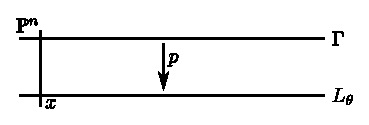
\includegraphics[scale=.8]{figures/chap1-fig1.eps}
\end{figure}

\subsubsection{}\label{chap1:5.6.1}
Let $\Lambda$ be the linear subsystem of $|B_{n}+(s+1)\ell|$
consisting of members which pass through $P_{0},\ldots,P_{m}$, $Q$
with multiplicities $\geqq 1$. Then we have the following:

\begin{lemma*}
With the notations as above, we have:
\begin{enumerate}
\renewcommand{\labelenumi}{\rm(\theenumi)}
\item $\Lambda$ is an irreducible linear pencil.

\item $S+\ell_{0}$ is a unique reducible member of $\Lambda$, and all
  other members of $\Lambda$ are nonsingular rational irreducible
  curves.

\item The proper transform $\Lambda'$ of $\Lambda$ by $\sigma$ has no
  base points; $E_{m+2}$ is a cross-section of the morphism
  $\Phi_{\Lambda'}:W\to \mathbb{P}^{1}$ defined by $\Lambda'$;
  $\sigma'(S)+E_{m+1}+E_{m}+\cdots+E_{1}+\sigma'(\ell_{0})$ is a
  member of $\Lambda'$.
\end{enumerate}
\end{lemma*}

\begin{proof}
Our proof consists of two steps.
\begin{enumerate}
\renewcommand{\theenumi}{\Roman{enumi}}
\renewcommand{\labelenumi}{(\theenumi)}
\item Since $\dim|B_{n}+(s+1)\ell|=2s-n+3=m+3$ we know that
  $\dim\Lambda\geqq m+3-(m+2)=1$. Let $D$ be a reducible member (if at
  all) of $\Lambda$ such that $D\neq S+\ell_{0}$, and write
  $D={\displaystyle{\mathop{\Sigma}^{t}_{i=1}}}n_{t}D_{t}$ with
  irreducible components $D_{i}$\pageoriginale\ and integers $n_{i}>0$
  for $1\leqq i\leqq t$. Then it is easy to see that one of $D_{i}$'s,
  say $D_{1}$, is linearly equivalent to $B_{n}+r\ell$ with $r\geqq 0$
  and $n_{1}=1$, and $D_{2},\ldots,D_{t}$ are fibers of the canonical
  projection $F_{n}\to \mathbb{P}^{1}$; we have $r\leqq s$ because $D$
  is a reducible member. Then, since $m\geqq 2$, $D_{1}$ must pass
  through the points $P_{0}$, $P_{1},\ldots,P_{m}$. This implies that
  $(D_{1}\cdot S)=s+r-n\geqq m+1=2s-n+1$, whence $r\geqq s+1$. This is
  a contradiction. Hence every member $D$ of $\Lambda$ such that
  $D\neq S+\ell_{0}$ is an irreducible curve. On the other hand, since
  $(D\cdot \ell)=1$ we know that $D$ is a nonsingular rational curve.

\item The fact that every number $D$ of $\Lambda$ such that $D\neq
  S+\ell_{0}$ is a nonsingular irreducible curve implies the
  following:
\begin{enumerate}
\renewcommand{\theenumii}{\roman{enumii}}
\renewcommand{\labelenumii}{(\theenumii)}
\item $\sigma'(S)+E_{m+1}+E_{m}+\cdots+E_{1}+\sigma'(\ell_{0})$ is a
  member of $\Lambda'$; hence $S+\ell_{0}$ is a (unique reducible)
  member of $\Lambda$.

\item Every member of $\Lambda'$ other than $\sigma'(S)+E_{m+1}+\cdots
  +E_{1}+\sigma'(\ell_{0})$ is of the form $\sigma'(D)$ with $D\in
  \Lambda$.
\end{enumerate}

Let $D$ and $D'$ be general members of $\Lambda$. Then, since $(D\cdot
D')=((B_{n}+(s+1)\ell)^{2})=2s-n+2=m+2$ we have $(\sigma'(D)\cdot
\sigma'(D'))=0$. This implies in turn the following:
\begin{enumerate}
\renewcommand{\theenumii}{\roman{enumii}}
\renewcommand{\labelenumii}{(\theenumii)}
\setcounter{enumii}{2}
\item $\Lambda'$ (hence $\Lambda$) is an irreducible linear pencil;
  $\Lambda'$ has no base points at all.

\item $E_{m+2}$ is a cross-section of the morphism
  $\Phi_{\Lambda'}:W\to \mathbb{P}^{1}$ defined by $\Lambda'$.
\end{enumerate}
\end{enumerate}

  The above observations complete the proof of Lemma (\ref{chap1:5.6.1}).
\end{proof}

\subsubsection{}\label{chap1:5.6.2}
Let\pageoriginale\ $\rho:W\to Z$ be the contraction of $\sigma'(S)$, $E_{m+1}$,
$E_{m},\ldots,E_{1}$ in this order, and let $T=\rho(E_{m+2})$. Since
$\rho$ contracts only curves in the member
$\sigma'(S)+E_{m+1}+\cdots+E_{1}+\sigma'(\ell_{0})$ of $\Lambda'$ we
know that the proper transform of $\Lambda'$ by $\rho$ defines a
structure of $\mathbb{P}^{1}$-bundle on $Z$, for which
$\rho(\sigma'(D))$ $(D\in \Lambda,D\neq S+\ell_{0})$ and
$\rho(\sigma'(\ell_{0}))$ constitute the fibers of the
$\mathbb{P}^{1}$-bundle $q:Z\to\mathbb{P}^{1}$, and $T$ is a
cross-section with $(T^{2})=m$. Note that $X=F_{n}-S$ is unchanged
under a birational transformation $\rho\cdot \sigma^{-1}:V\to
Z$. Consequently, $X$ has a structure of $\mathbb{A}^{1}$-bundle
$g:X\to \mathbb{P}^{1}$ other than $f:X\to \mathbb{P}^{1}$, where
$X=Z-T$ and $g:=q|_{X}$. However, we could not determine integers $n'$
and $s'$ such that $Z=F_{n'}$, and $T\sim B_{n'}+s'\ell$.

\subsection{}\label{chap1:5.7}
In this paragraph we shall show that the affine surface
$X=F_{n}-S_{\infty}$ constructed in \ref{chap1:5.2} has a nontrivial
$G_{a}$-action. With the notations of \ref{chap1:5.6}, choose a point
$P_{0}$ so that $P_{0}\not\in S_{\infty}\cap B_{n}$ if $n>0$. Take the
points $P_{1},\ldots,P_{m-1}$ as in \ref{chap1:5.6}, and let
$\sigma_{i}:V_{i}\to V_{i-1}$ be a quadratic transformation with
center at $P_{i-1}$ for $1\leqq i\leqq m$, where $V_{0}:=V$. Let
$\varphi=\sigma_{1}\cdot\ldots\cdot\sigma_{m}$, and let
$E_{i}=(\sigma_{i+1}\cdot\ldots\cdot\sigma_{m})'(\sigma^{-1}_{i}(P_{i-1}))$,
by abuse of notations, for $1\leqq i<m$ and
$E_{m}=\sigma^{-1}_{m}(P_{m-1})$. 

\subsubsection{}\label{chap1:5.7.1}
Let $N$ be the linear subsystem of $|B_{n}+(s-1)\ell|$ consisting of
members which pass through the points $P_{0},P_{1},\ldots,P_{m-2}$
with multiplicities $\geqq 1$. Then we have:

\begin{lemma*}
With the notations as above, $M$ consists of a single member $T$ which
is a nonsingular rational irreducible curve. 
\end{lemma*}

\begin{proof}
Since\pageoriginale\ $\dim|B_{n}+(s-1)\ell|=2s-n-1=m-1$, we have $\dim
M\geqq (m-1)-(m-1)=0$. Hence $M$ is not empty. Let $D$ be a member of
$M$. We shall show that $D$ is an irreducible curve. Assume the
contrary, and write
$D={\displaystyle{\mathop{\Sigma}^{t}_{i=1}}}n_{i}D_{i}$ with
irreducible components $D_{i}$ and integers $n_{i}>0$ for $1\leqq
i\leqq t$. Then, as in the proof of Lemma \ref{chap1:5.6.1}, one of
$D_{i}$'s, say $D_{1}$, is linearly equivalent to $B_{n}+r\ell$ with
$r\geqq 0$ and $n_{1}=1$, and $D_{2},\ldots,D_{t}$ are fibers of the
canonical projection $F_{n}\to \mathbb{P}^{1}$. Then we have $r\leqq
s-2$ since $D$ is reducible, whence $s\geqq 2$ and $m\geqq 3$. Then
$D_{1}$ must pass through the points
$P_{0},P_{1},\ldots,P_{m-2}$. This implies that $(D_{1}\cdot
S)=s+r-n\geqq m-1=2s-n-1$, whence $r\geqq s-1$. This is a
contradiction. Thus every member $D$ of $M$ is irreducible. On the
other hand, since $(D\cdot\ell)=1$ we know that $D$ is a nonsingular
rational curve. If $\dim M>0$, let $D$ and $D'$ be general members of
$M$. Then $(D\cdot D')=((B_{n}+(s-1)\ell)^{2})=2s-n-2=m-2$ while
$(D\cdot D')$ must be $\geqq m-1$. This is a contradiction. Hence
$\dim M=0$.
\end{proof}

\subsubsection{}\label{chap1:5.7.2}
Let $M$ be the linear subsystem of $|B_{n}+s\ell|$ consisting of
members which pass through the points $P_{0},P_{1},\ldots,P_{m-1}$
with multiplicities $\geqq 1$. Then we have:

\begin{lemma*}
With the notations as above, we have:
\begin{enumerate}
\renewcommand{\labelenumi}{\rm(\theenumi)}
\item $N$ is an irreducible linear pencil.

\item $T+\ell_{0}$ is a unique reducible member of $N$, and all other
  members of $N$ are nonsingular rational irreducible curves.

\item The proper transform $N'$ of $N$ by $\varphi$ has no base
  points; $E_{m}$ is a cross-section of the morphism
  $\Phi_{N'}:V_{m}\to \mathbb{P}^{1}$ defined by $N'$;\pageoriginale\
  $\varphi'(T)+E_{m-1}+\cdots+E_{1}+\varphi'(\ell_{0})$ is a member of $N'$.
\end{enumerate}
\end{lemma*}

\begin{proof}
All assertions can be proved in the same fashion as in the proof of
\ref{chap1:5.6.1} with slight modifications. Therefore we shall leave a
proof to readers as an exercise.
\end{proof}

\subsubsection{}\label{chap1:5.7.3}
We have the following configuration of $\varphi^{-1}(S\cup T\cup
\ell_{0})$:
\begin{figure}[H]
\centering
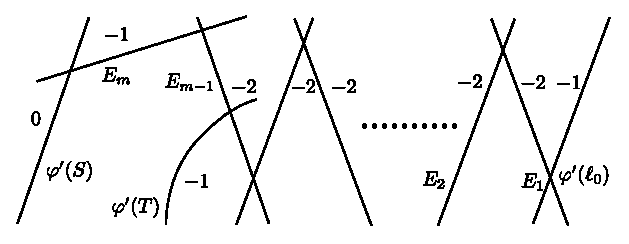
\includegraphics{figures/chap1-fig2.eps}
\end{figure}

Note that $X=V_{m}-(\varphi'(S)\cup E_{m}\cup\ldots\cup E_{1})$ and
$V_{m}$ has a linear pencil $N'$ whose members are $\varphi'(D)$'s for
$D\in N$ with $D\neq T+\ell_{0}$ and $\varphi'(T)+E_{m-1}+\cdots
+E_{1}+\varphi'(\ell_{0})$. Therefore, it is easily seen that the
affine surface $X$ has an algebraic pencil $\mathscr{F}$ of affine
lines parametrized by the affine line $\mathbb{A}^{1}$. Let $Q_{0}$ be
the point on $\mathbb{A}^{1}$ corresponding to the member
$(\varphi'(T)\cup \varphi'(\ell_{0}))\cap X$. Then
$X_{0}:=X-(\varphi'(T)\cup \varphi'(\ell_{0}))$ has an algebraic
pencil of affine lines parametrized by
$\mathbb{A}^{1}_{\ast}:=\mathbb{A}^{1}-\{Q_{0}\}$, where every member
of the pencil is the affine line. Hence $X_{0}$ is an
$\mathbb{A}^{1}$-bundle over $\mathbb{A}^{1}_{\ast}$, which is
trivial, \iec $X_{0}\cong \mathbb{A}^{1}\times
\mathbb{A}^{1}_{\ast}$. Then, as in Lemma \ref{chap1:2.2.1} and Theorem
\ref{chap1:2.3}, we can readily show that there exists a nontrivial
$G_{a}$-action on $X$ such that every member of $\mathscr{F}$ other
than $(\varphi'(T)\cup \varphi'(\ell_{0}))\cap X$ is the
$G_{a}$-orbit.

\section[Locally nilpotent........]{Locally nilpotent derivations in connection with the
  cancellation problem}\label{chap1:sec6}\pageoriginale\

\subsection{}\label{chap1:6.1} 
A $k$-algebra $A$ is called {\em strongly}
$n$-{\em invariant} (or $n$-{\em invariant}) if $A$ satisfies the
condition: Given a $k$-algebra $B$ and indeterminates
$X_{1},\ldots,X_{n}$ and $Y_{1},\ldots,Y_{n}$, if
$\theta:A[X_{1},\ldots,X_{n}]\xrightarrow{\sim}B[Y_{1},\ldots,Y_{n}]$
is a $k$-isomorphism then we have necessarily $\theta(A)=B$ (or $A$ is
isomorphic to $B$ under some $k$-isomorphism). If $A$ is strongly
$n$-invariant (or $n$-invariant) for all integers $n\geqq 1$ then $A$
is called {\em strongly invariant} (or {\em invariant}). A problem
asking whether or not a (given) $k$-algebra $A$ is strongly invariant
(or invariant) is called, in general, the cancellation problem. The
purpose of this section is to apply the results in the previous
sections to the cancellation problem. Namely, we are interested in
looking for necessary or sufficient conditions for a given $k$-algebra
to be strongly invariant, which can be written in terms of locally
finite (or locally finite iterative) higher derivations.

\subsection{}\label{chap1:6.2}
A sufficient condition for strong $1$-invariance is given, by making
use of Nagata's theorem \cite{42}, in the following:

\begin{lemma*}[(\cf \cite{1}) ]
Let $A$ be an affine $k$-domain. If $A$ is not birationally ruled over
$k$, then $A$ is strongly $1$-invariant.
\end{lemma*}

Here, an affine $k$-domain $A$ is said to be {\em birationally ruled
  over} $k$ if the quotient field $Q(A)$ is a purely transcendental
extension $K(t)$ in one variable over a sub field $K$ of $Q(A)$
containing $k$. 

\subsection{}\label{chap1:6.3}
Another\pageoriginale\ sufficient condition for strong invariance is
the following:

\begin{lemma*}
Let $A$ be a $k$-algebra. If $A$ has no nontrivial locally finite
higher derivations then $A$ is strongly invariant.
\end{lemma*}

\begin{proof}
\footnote{We are indebted to $Y$. Ishibashi for improving the original
proof.} 
Assume that $A$ is not strongly invariant. Then there exists a
$k$-algebra $B(\neq A)$ such that
$A[X_{1},\ldots,X_{n}]=B[Y_{1},\ldots,Y_{n}]$ for some integer $n\geqq
1$, where $X_{1},\ldots,X_{n}$ and $Y_{1},\ldots,Y_{n}$ are
algebraically independent over $A$ and $B$, respectively. Let $a$ be
an element of $A$ not in $B$. Then $a$ is written as
$$
a=\Sigma b_{\alpha_{1}\ldots\alpha_{n}}Y^{\alpha_{1}}_{1}\ldots
Y^{\alpha_{n}}_{n}=f(Y_{1},\ldots,Y_{n})\not\in B.
$$
Assume that $Y_{1}$ appears in $f(Y_{1},\ldots,Y_{n})$. Let $T$ be an
indeterminate and let $\psi$ be a $k$-algebra homomorphism of
$B[Y_{1},\ldots,Y_{n}]$ into $B[Y_{1},\ldots$, $Y_{n},T]$ such that
$\psi(Y_{1})=Y_{1}+T$ and $\psi(Y_{i})=Y_{i}$ for $2\leqq i\leqq
n$. Then we can see easily that $\psi(a)$ is written as
$$
\psi(a)=a+T^{m}g(Y_{1},\ldots,Y_{n},T)~\text{with}~
g(Y_{1},\ldots,Y_{n},T)\neq 0~\text{and}~ m\geqq 1.
$$
Write $g(Y_{1},\ldots,Y_{n},T)=h(X_{1},\ldots,X_{n},T)\in
A[X_{1},\ldots,X_{n},T]$.\break Let $\mu_{1},\ldots$, $\mu_{n}$ be a set of
positive integers such that $h(T^{\mu_{1}},\ldots,T^{\mu_{n}},T)\neq
0$. Let 2 be the canonical injection $A\hookrightarrow
A[X_{1},\ldots,X_{n}]$ and let $\tau$ be a homomorphism (of
$A$-algebras) of $A[X_{1},\ldots,X_{n},T]=B[Y_{1},\ldots,Y_{n},T]$
into $A[T]$ such that $\tau(X_{i})=T^{\mu_{i}}$ for $1\leqq i\leqq n$
and $\tau(T)=T$. Let $\rho=\tau\cdot\psi\cdot 2$. Then $\rho$ is a
$k$-algebra homomorphism of $A$ into $A[T]$ such that $\rho(a)\not\in
A$ and $\rho$ defines a nontrivial locally\pageoriginale\ finite higher derivation
(\cf Lemma \ref{chap1:1.2}).
\end{proof}

\subsection{}\label{chap1:6.4}
As a practical criterion for strong invariance, the next result given
in \ref{chap1:6.4.1} below is often more useful than the one given in Lemma
\ref{chap1:6.3}. 

\subsubsection{}\label{chap1:6.4.1}
\begin{lemma*}
  Let $k$ be an infinite field and let $A$ be an affine $k$-domain
  satisfying the conditions:
  \begin{enumerate}
    \renewcommand{\labelenumi}{\rm (\theenumi)}
  \item $\Spec(A)(k)$ is dense in $\Spec (A)$.
    
  \item There is no nonconstant $k$-morphism from the affine line
    $\mathbb{A}^{1}_{k}$ to $\Spec (A)$.
  \end{enumerate}
  Then $A$ is strongly invariant.
\end{lemma*}

The proof can be done along the same principle as in the proof of
Lemma \ref{chap1:6.3}, and we shall leave it to readers.


\subsubsection{}\label{chap1:6.4.2}
The rings in the next two examples can be shown to be strongly
invariant by applying Lemma \ref{chap1:6.4.1}, the first one of which was
first given by Hochster \cite{23} and discussed later by Eakin and
Heinzer \cite{13}.

\begin{example*}[1 ]
Let
$A_{n}:=\mathbb{R}[X_{0},\ldots,X_{n}]/(X^{2}_{0}+\cdots+X^{2}_{n}-1)$
be the affine ring of the real $n$-sphere for $n\geqq 1$. Then $A_{n}$
is strongly invariant; a polynomial ring $A_{n}[t]$ in one variable
over $A_{n}$ is invariant; a polynomial ring
$A_{n}[t_{1},\ldots,t_{n}]$ in $n$-variables over $A_{n}$ is not
$1$-invariant if $n\neq 1,3,7$.
\end{example*}

\begin{example*}[2 ]
Let $k$ be a non-perfect field of characteristic $p>0$, and let
$A=k[X,Y]/(Y^{p^{n}}-X-a_{1}X^{p}-\ldots-a_{r}X^{p^{r}})$, where $r$,
$n>0$ and $a_{1},\ldots,a_{r}\in k$ with one of
$a_{1},\ldots,a_{r}\not\in k^{p}$. A is the affine\pageoriginale\ ring
of a Russell $k$-group, which will be discussed in Chapter III. Then
$A$ is strongly invariant, while, for the perfect closure $k'$ of $k$,
$\foprod{A}{k'}{k}$ is not strongly invariant because
$\foprod{A}{k'}{k}$ is a polynomial ring in one variable over $k'$.

The second example exhibits that strong invariance is not preserved
under faithfully flat ascent, while it is preserved under faithfully
flat descent (\cf Miyanishi and Nakai \cite{36}).
\end{example*}

\subsubsection{}\label{chap1:6.4.3}
The converse of Lemma \ref{chap1:6.3} does not hold as shown by the next 

\begin{example*}
Let $k$ be an algebraically closed field and let $A$ be the affine
ring of the affine cone of a nonsingular projective variety
$U$. Assume that there is no nonconstant $k$-rational mapping from
$\mathbb{A}^{1}_{k}$ to $U$. Then $A$ is strongly invariant, while $A$
has a nontrivial locally finite higher derivation.
\end{example*}

\begin{proof}
As shown in \ref{chap1:2.2.3}, $A$ has a nontrivial locally finite higher
derivation. Hence it remains to show that $A$ is strongly
invariant. Assume that we are given a $k$-algebra $B$ satisfying
$A[X_{1},\ldots,X_{n}]=B[Y_{1},\ldots,Y_{n}]$, where
$X_{1},\ldots,X_{n}$ and $Y_{1},\ldots,Y_{n}$ are algebraically
independent over $A$ and $B$, respectively. Set $V:=\Spec (A)$ and
$W:=\Spec(B)$; $W$ (as well as $V$) is an affine variety defined over
$k$ because the relation $A[X_{1},\ldots,X_{n}]=B[Y_{1},\ldots,Y_{n}]$
implies that $B$ is an affine $k$-domain; we have $V\times
\mathbb{A}^{n}_{k}=W\times\mathbb{A}^{n}_{k}$. Let $q_{V}:V\times
\mathbb{A}^{n}_{k}\to V$ and $q_{W}:W\times\mathbb{A}^{n}_{k}\to W$ be
the canonical projections onto $V$ and $W$, respectively, and let
$\pi:V-\{v_{0}\}\to U$ be the projection of the cone to the base
variety, where $v_{0}$ is the vertex\pageoriginale\ of the cone
$V$. For a point $w$ of $W$, $\pi q_{V}(q^{-1}_{W}(w))$ is a point $u$
of $U$ because of the stated assumption that there is no nonconstant
$k$-rational mapping of $\mathbb{A}^{1}_{k}$ to $U$. Assume that
$q_{V}(q^{-1}_{W}(w))$ is not a point. Then
$q_{V}(q^{-1}_{W}(w))=\pi^{-1}(u)$ because $q_{V}(q^{-1}_{W}(w))$ is
an affine rational curve with only one place at infinity and
$q_{V}(q^{-1}_{W}(w))\subset \pi^{-1}(u)$. This implies that
$q^{-1}_{W}(w)$ intersects the singular locus $q^{-1}_{V}(v_{0})$ of
$V\times \mathbb{A}^{n}_{k}=W\times\mathbb{A}^{n}_{k}$. Besides, it is
readily shown that $W$ has a unique singular point $w_{0}$ and
$q^{-1}_{W}(w_{0})$ is the singular locus of $W\times
\mathbb{A}^{n}_{k}$; hence
$q^{-1}_{V}(v_{0})=q^{-1}_{W}(w_{0})$. Thus, we have $w=w_{0}$ because
$q^{-1}_{W}(w)\cap q^{-1}_{W}(w_{0})\neq \phi$. If $w\neq w_{0}$ we
have shown that $q_{V}(q^{-1}_{W}(w))$ is a point $v$ of $V$, \iec
$q^{-1}_{W}(w)\subset q^{-1}_{V}(v)$. Indeed, we have
$q^{-1}_{W}(w)=q^{-1}_{V}(v)$ because both $q^{-1}_{W}(w)$ and
$q^{-1}_{V}(v)$ are isomorphic to $\mathbb{A}^{n}_{k}$ (\cf Ax
\cite{8}). This means that every maximal ideal of $B$ is vertical
relative to $A$ in the terminology of \cite{1}. Then $A=B$ by virtue
of [ibid., (1.13)].
\end{proof}

\subsection{}\label{chap1:6.5}
A necessary condition for strong invariance is given by the next

\begin{lemma*}
Let $A$ be a $k$-algebra. If $A$ has a nontrivial locally finite
iterative higher derivation $D$ then $A$ is not strongly $1$-invariant.
\end{lemma*}

\begin{proof}
Let $\varphi:A\to A[t]$ be the $k$-homomorphism associated with $D$
(\cf \ref{chap1:1.2}). Let $B=\varphi(A)$. We shall show that
$A[t]=B[t]$. Since $B[t]\subseteq A[t]$, we have only to show the
following assertion by induction on $n$:
\begin{quote}
$P(n):$~If\pageoriginale\ $a$ is an element of $A$ with
  $D$-length $\ell(a)=n$ (\cf \ref{chap1:1.4}) then $a\in B[t]$.
\end{quote}
If $\ell(a)=0$ then $a=\varphi(a)\in B$. Assume that $\ell(a)=n>0$ and
$P(r)$ is true for $0\leqq r<n$. Since $\ell(D_{i}(a)<n)$ for $i\geqq
1$ we have $D_{i}(a)\in B[t]$ by virtue of $P(r)$ for $r<n$. Then,
since $a=\varphi(a)-{\displaystyle{\mathop{\Sigma}_{i\geqq
      1}}}D_{i}(a)t^{i}$ we have $a\in B[t]$. Thus, $P(n)$ is proved,
and $A$ is not strongly $1$-invariant.
\end{proof}

\subsection{}\label{chap1:6.6}
In the paragraphs \ref{chap1:6.6} and \ref{chap1:6.7} we shall consider whether or
not the converse of Lemma \ref{chap1:6.6} is true. When $A$ is an affine
$k$-domain of dimension $1$, this is true and was essentially proved
in [1; (3.4)]. We have in fact:

\subsubsection{}\label{chap1:6.6.1}
\begin{prop*}
  Let $A$ be an affine $k$-domain of dimension $1$. Then the following
  conditions are equivalent to each other:
  \begin{enumerate}
    \renewcommand{\labelenumi}{\rm(\theenumi)}
  \item $A$ is strongly invariant.
    
  \item $A$ is strongly $1$-invariant.
    
  \item $A$ has no nontrivial locally finite iterative higher derivation.
  \end{enumerate}
\end{prop*}

\begin{proof}
(1) $\Longrightarrow$ (2) is clear; (2) $\Longrightarrow$ (3) follows
  from Lemma \ref{chap1:6.5} and its proof. (3) $\Longrightarrow$ (1): It
  is proved in [1; (3.4)] that under the stated assumption $A$ is
  either strongly invariant or $A$ is a polynomial ring $k_{0}[x]$
  over the algebraic closure $k_{0}$ of $k$ in $A$. In the latter case
  $A$ has a nontrivial locally finite iterative higher
  derivation. Thus we have (3) $\Longrightarrow$ (1).
\end{proof}

\subsubsection{}\label{chap1:6.6.2}
When\pageoriginale\ $\dim A=2$ we have the following:

\begin{prop*}
Let $k$ be an algebraically closed field of characteristic zero, and
let $A$ be an irrational nonsingular affine $k$-domain of dimension
$2$. Then we have one of the following three cases:
\begin{enumerate}
\renewcommand{\labelenumi}{\rm(\theenumi)}
\item $A$ is strongly $1$-invariant.

\item $A$ has a nontrivial locally finite iterative higher derivation.

\item There is a surjective morphism $\pi:\Spec(A)\to C$ from
  $\Spec(A)$ to a nonsingular complete curve $C$ of genus $>0$, whose
  general fibers are isomorphic to the affine line $\mathbb{A}^{1}_{k}$.
\end{enumerate}
\end{prop*}

\begin{proof}
Assume that $A$ is not strongly $1$-invariant. Then, by virtue of
Lemma \ref{chap1:6.2}, $A$ is birationally ruled. Set
$V:=\Spec(A)$. Since $A$ is irrational the irregularity $g$ of $V$ is
positive; the Albanese mapping of a nonsingular
completion\footnote{Note that $\pi$ does not depend on choices of
  nonsingular completions of $V$.}
of $V$ induces a unique morphism $\pi:V\to C$, where $C=\pi(V)$ and
$C$ is a nonsingular (not necessarily complete) curve of genus $g>0$;
the general fibers of $\pi$ are irreducible rational curves. On the
other hand, since $A$ is not strongly $1$-invariant there exists an
affine $k$-domain $B(\neq A)$ of dimension $2$ such that $A[X]=B[Y]$,
where $X$ and $Y$ are algebraically independent over $A$ and $B$,
respectively. Set $W:=\Spec(B)$, and let $q_{V}:V\times
\mathbb{A}^{1}_{k}\to V$ and $q_{W}:W\times\mathbb{A}^{1}_{k}\to W$ be
the canonical projections from
$V\times\mathbb{A}^{1}_{k}=W\times\mathbb{A}^{1}_{k}$ to $V$ and $W$,
respectively.\pageoriginale\ For a general point $w$ of $W$,
$\ell_{w}:=q_{V}(q^{-1}_{W}(w))$ is an affine rational curve with only
one place at infinity. Indeed, if $q_{V}(q^{-1}_{W}(w))$ is a point
$v$ on $V$ then $q^{-1}_{V}(v)=q^{-1}_{W}(w)$; if
$q^{-1}_{W}(w)=q^{-1}_{V}(v)$ for every point $w$ of $W$ and a point
$v$ of $V$ (depending on $w$) every maximal ideal of $B$ is vertical
relative to $A$, whence $A=B$ (\cf [1; (1.13)]); thus
$q_{V}(q^{-1}_{W}(w))$ is not a point for some point $w$ of $W$ and,
{\em a fortiori}, for a general point of $W$. Since $\pi(\ell_{w})$ is
a point on $C$ we know that $\ell_{w}$ is contained in a fiber of
$\pi$; since a general fiber of $\pi$ is irreducible $\ell_{w}$
coincides with a fiber of $\pi$ for a general point $w$ of
$W$. Moreover, since the morphism $\pi:V\to C$ defines an irrational
pencil on $V$ and since an irrational pencil on a nonsingular surface
has no base points, the second theorem of Bertini's tells us that
$\ell_{w}$ is isomorphic to the affine line. consequently, we know
that the morphism $\pi:V\to C$ is an algebraic pencil of affine lines
parametrized by the curve $C$ (\cf Section \ref{chap1:sec2}). If $C$
is not complete, set $A_{0}:=k[C]$. Then $A_{0}$ is a $k$-subalgebra
of $A$ of dimension $1$, and we have a nontrivial $G_{a}$-action on
$V$ with respect to which the general fibers of $\pi$ are
$G_{a}$-orbits (\cf Lemma \ref{chap1:2.2.1} and Theorem
\ref{chap1:2.3}). Thus we are reduced to the case (2). If $C$ is a
complete curve then we are reduced to the case (3).
\end{proof}

\subsubsection{}\label{chap1:6.6.3}
\begin{lemma*}
  Let $k$ be an algebraically closed field of characteristic zero and
  let $V$ be a nonsingular affine surface defined over $k$. Assume that
  there exists a surjective morphism $\pi:V\to C$ from $V$ onto a
  nonsingular complete curve $C$, whose general fibers\pageoriginale\ are
  isomorphic to the affine line. Then we have:
  \begin{enumerate}
    \renewcommand{\labelenumi}{\rm(\theenumi)}
  \item Every irreducible component of a fiber of $\pi$ is isomorphic to
    the affine line; if a fiber is reducible every irreducible component
    is a connected component.
    
  \item There exist a nonsingular projective surface $\widetilde{V}$ and
    a surjective morphism $\widetilde{\pi}:\widetilde{V}\to C$ such
    that:
    \begin{enumerate}
      \renewcommand{\theenumii}{\roman{enumii}}
      \renewcommand{\labelenumii}{\rm(\theenumii)}
    \item $\widetilde{V}$ contains $V$ as an open set, and
      $\widetilde{\pi}|_{V}=\pi$, 
      
    \item general fibers of $\widetilde{\pi}$ are isomorphic to the
      projective line $\mathbb{P}^{1}_{k}$,
      
    \item $\widetilde{V}-V$ consists of a cross-section $S$ and
      irreducible components contained in several reducible fibers of
      $\widetilde{\pi}$. 
    \end{enumerate}
  \end{enumerate}
\end{lemma*}

\begin{proof}
Let $\widetilde{V}$ be a nonsingular projective surface containing $V$
as an open set. Then the morphism $\pi:V\to C$ defines an irreducible
pencil $\Lambda$ on $\widetilde{V}$, whose base points (if at all) lie
on $\widetilde{V}-V$. By replacing $\widetilde{V}$ (if necessary) by
the surface which is obtained from $\widetilde{V}$ by a succession of
quadratic transformations with centers at base points (including
infinitely near base points) of $\Lambda$, we may assume that
$\Lambda$ has no base points. Let $\widetilde{\pi}:\widetilde{v} \to C 
$. Since a general fiber $\ell$ of $\pi$ is isomorphic to
$\mathbb{A}^{1}_{k}$ and the characteristic of $k$ is zero, we know
that a general fiber of $\widetilde{\pi}$ is isomorphic to
$\mathbb{P}^{1}_{k}$ and $\ell$ is of the form:
$\ell=\widetilde{\ell}-\widetilde{\ell}\cap S$, where
$\widetilde{\ell}\cong \mathbb{P}^{1}_{k}$, $S$ is a cross-section of
$\widetilde{\pi}$ and $(\widetilde{\ell}\cdot S)=1$. Then all
assertions stated in the lemma are readily verified by looking at the
fibration $\widetilde{\pi}:\widetilde{V}\to C$ and taking into account
that $V$ is an affine open set of $\widetilde{V}$, (see Chapter \ref{chap2},
Section \ref{chap2:sec2}).
\end{proof}

\subsubsection{}\label{chap1:6.6.4}
In\pageoriginale\ the case (3) of Proposition \ref{chap1:6.6.2} the
surface $V:=\Spec(A)$ has a structure as described in Lemma
\ref{chap1:6.6.3}. We have an impression that $A$ is strongly
$1$-invariant in this case. As an evidence we shall prove in the next
paragraph that $A$ is strongly $1$-invariant in the simplest case;
namely the case where every fiber of $\pi$ is irreducible (\cf Theorem
\ref{chap1:4.9} and Lemma \ref{chap1:5.2}).


\subsection{}\label{chap1:6.7}
\begin{prop*}
Let $k$ be an algebraically closed field of characteristic zero, let
$C$ be a nonsingular complete curve of genus $g>0$ defined over $k$,
let $L$ be an ample line bundle over $C$ and let $E$ be a nontrivial
extension of $L$ by $\mathscr{O}_{C}$. Let $X$ be the
$\mathbb{P}^{1}$-bundle $\mathbb{P}(E)$ minus the section $S$
corresponding to $L$ and let $A$ be the affine ring of $X$. Then $A$
is strongly $1$-invariant.
\end{prop*}

\subsubsection{}\label{chap1:6.7.1}
In order to prove this result we need the next

\begin{lemma*}
Let $k$ be a field of characteristic zero and let $\varphi$ be a
$k$-automor\-phism of a polynomial ring $k[x,y]$ in two variables $x$,
$y$ over $k$. Assume that $\varphi$ is given by $\varphi(x)=f$ and
$\varphi(y)=g$ with $f$, $g\in k[x,y]$. Then $f$ has the following
form unless $f$ is a polynomial in $x$ or $y$ alone:
\begin{equation*}
f=ax^{m}+by^{n}+\sum_{\substack{m>i\\ n>j}}c_{ij}x^{i}y^{j},\tag{*}
\end{equation*}
where $a$, $b$ and $c_{ij}$'s are elements of $k$ and $ab\neq 0$. The
same assertion holds for $g$.
\end{lemma*}

\begin{proof}
Our proof consists of four steps.
\begin{enumerate}
\renewcommand{\theenumi}{\Roman{enumi}}
\renewcommand{\labelenumi}{(\theenumi)}
\item First\pageoriginale\ we shall treat the case where one of $f$ and
  $g$, say $f$, is a polynomial in either one only of variables $x$
  and $y$, say $y$. Since $\varphi$ is a $k$-automorphism of $k[x,y]$
  the Jacobian determinant $\left|\dfrac{\partial(f,g)}{\partial
    (x,y)}\right|=-\left(\dfrac{\partial f}{\partial
    y}\right)\left(\dfrac{\partial g}{\partial x}\right)$ is a nonzero
  constant in $k$. Hence $\dfrac{\partial f}{\partial y}=a$ and
  $\dfrac{\partial g}{\partial x}=b$ are also nonzero constants in
  $k$. Thence we may write: $f=ay+c$ and $g=bx+h(y)$ with $c\in k$ and
  $h(y)\in k[y]$.

\item Assume that $f$ has the form $(\ast)$ and $g$ is not a
  polynomial in $x$ or $y$ alone. Then we shall show that $g$ has also
  the form $(\ast)$. Write
$$
g=\alpha_{0}(y)x^{u}+\alpha_{1}(y)x^{u-1}+\cdots+\alpha_{u}(y)\quad
(\alpha_{0}(y)\neq 0, u>0) 
$$
where $\alpha_{i}(y)\in k[y]$. Since $\left|\dfrac{\partial
  (f,g)}{\partial(x,y)}\right|$ is a nonzero constant in $k$ we can
easily ascertain that the first derivative $\alpha'_{0}(y)$ is
zero. Hence $\alpha_{0}(y)$ is a nonzero constant in $k$. Similarly if
we write $g$ in the form
$$
g=\beta_{0}(x)y^{v}+\beta_{1}(x)y^{v-1}+\cdots+\beta_{v}(y)\quad
(\beta_{0}(x)\neq 0, v>0),
$$
we have $\beta_{0}(x)\in k$. These facts imply that $g$ has the form
$(\ast)$ 

\item It is known (\cf Chapter II, Section 3; also \cite{43}) that any
  $k$-auto\-morphism of $k[x,y]$ is a composite of linear automorphisms
  of type $(x,y)\mapsto (\alpha x+\beta y+c,\gamma x+\delta y+d)$ with
  $\alpha\delta-\beta\gamma\neq 0$ and de Jonqui\`ere automorphisms of
  type $(x,y)\mapsto (x,y+h(x))$ with $h(x)\ominus k[x]$. Using this
  fact we shall show that any $k$-automorphism of $k[x,y]$ is a
  composite of automorphisms, each of which is an automorphism $\rho$
  such that $\rho(x)$ or $\rho(y)$ coincides with one of $x$
  and\pageoriginale\ $y$. We shall say such an automorphism to be of
  type $(P)$. Since a de Janqui\`ere automorphism is obviously of type
  $(P)$ it suffices to show that a linear automorphism is a composite
  of linear automorphism $(P)$. Indeed, a linear automorphism
  $(x,y)\mapsto (\alpha x+\beta y+c,\gamma x+\delta y+d)$ is
  decomposed as follows: If $\alpha\neq 0$, $(x,y)\mapsto
  (x',y')=(\alpha x+\beta y+c, y)$, $(x',y')\mapsto
  (x',(\gamma/\alpha)x'+((\alpha
  \delta-\beta\gamma)/\alpha)y'+(d-(\gamma c/\alpha)))$; if
  $\alpha=0$, $(x,y)\mapsto (x',y')=(y,\gamma x+\delta y+d)$,
  $(x',y')\mapsto
  (((\beta\gamma-\alpha\delta)/\gamma)x'+(\alpha/\gamma)y'+(c-(\alpha
  d/\gamma)),y')$. 

\item Write the given automorphism $\varphi$ as
  $\varphi=\varphi_{r}\cdot \varphi_{r-1}\cdot\ldots\cdot
  \varphi_{1}$, where $\varphi_{1},\ldots,\varphi_{r}$ are
  automorphisms of type $(P)$. We shall prove our assertion by
  induction on $r$. If $r=1$, $\varphi$ has one of the following
  forms: $(x,y)\mapsto (ax+h(y),y)$, $(x,y)\mapsto
  (y,a_{1}x+h_{1}(y))$, $(x,y)\mapsto (x,by+\ell(x))$ or $(x,y)\mapsto
  (b_{1}y+\ell_{1}(x),x)$, where $a$, $a_{1}$, $b$, $b_{1}\in k$,
  $h(y)$, $h_{1}(y)\in k[y]$ and $\ell(x)$, $\ell_{1}(x)\in
  k[x]$. Hence the assertion holds clearly. Assuming that the
  assertion is true when $\varphi$ is a composition of less than $r$
  automorphisms of type $(P)$ we shall consider the case where
  $\varphi=\varphi_{r}\cdot
  \varphi_{r-1}\cdot\ldots\cdot\varphi_{1}$. Let
  $\psi=\varphi_{r-1}\cdot\ldots\cdot\varphi_{1}$, and let
  $(\psi(x),\psi(y))=(f_{1},g_{1})$ with $f_{1}$, $g_{1}\in
  k[x,y]$. By the assumption of induction $f_{1}$ and $g_{1}$ have the
  form $(\ast)$ unless they are polynomials in $x$ or $y$ alone. Since
  $\varphi_{r}$ is an automorphism of type $(P)$ we have one of the
  following cases:
\begin{center}
  (i)~$\varphi(x)=f_{1}$,\quad (ii)~$\varphi(x)=g_{1}$,\quad
  (iii)~$\varphi(y)=f_{1}$,\quad (iv)~$\varphi(y)=g_{1}$.
\end{center}
In any case we can easily ascertain the truth of our assertion in
virtue of steps (I) and (II).
\end{enumerate}
\end{proof}

\subsubsection{}\label{chap1:6.7.2}\pageoriginale\
\begin{proofofprop*}
Our proof consists of three steps.
\begin{enumerate}
\renewcommand{\theenumi}{\Roman{enumi}}
\renewcommand{\labelenumi}{(\theenumi)}
\item Let $B$ be a $k$-algebra such that $A[T]=B[V]$, where $T$ and
  $V$ are algebraically independent over $A$ and $B$,
  respectively. Set $Y:=\Spec(B)$, and let $\pi:X\to C$ be the
  restriction onto $X$ of the canonical projection $\mathbb{P}(E)\to
  C$. By a composition of projections $Y\times
  \mathbb{A}^{1}_{k}=X\times\mathbb{A}^{1}_{k}\xrightarrow{p_{1}}X\xrightarrow{\pi}C$,
  each line $(y)\times\mathbb{A}^{1}_{k}$ with $y\in Y$ is sent to a
  point of $C$. Hence $\pi\cdot p_{1}$ factors as
  $Y\times\mathbb{A}^{1}_{k}\xrightarrow{p'_{1}}Y\xrightarrow{q}C$,
  and $Y$ is viewed as a $C$-scheme by means of $q$. Note that $q$ is
  surjective. Let $\mathscr{U}=\{U_{i}\}_{i\in I}$ be an affine open
  covering of $C$ such that $E|_{U_{i}}$ is trivial for every $i\in
  I$. Let $\{x_{i}\}_{i\in I}$ be an affine coordinate system of $X$
  relative to $\mathscr{U}$; $\{x_{i}\}_{i\in I}$ is subject to
  $x_{j}=a_{ji}x_{i}+b_{ji}$ with $a_{ji}\in R^{\ast}_{ij}$ and
  $b_{ji}\in R_{ij}$, where $R_{ij}:=k[U_{i}\cap U_{j}]$. Set
  $R_{i}:=k[U_{i}]$ and $B_{i}:=k[q^{-1}(U_{i})]$. Then we have
  $R_{i}[x_{i},T]=B_{i}[V]$ for every $i\in I$. Since $B_{i}$ is an
  $R_{i}$-algebra and $R_{i}$ is regular there is an element $y_{i}\in
  B_{i}$ such that $B_{i}=R_{i}[y_{i}]$ (\cf [1; (4.7)]). This implies
  that $q:Y\to C$ is an $\mathbb{A}^{1}$-bundle over $C$ (\cf
  \ref{chap1:4.9}). Hence by virtue of Lemma \ref{chap1:5.2} there exist an
  ample line bundle $L'$ over $C$ and a nontrivial extension $E'$ of
  $L'$ by $\mathscr{O}_{C}$ such that $Y$ is $C$-isomorphic to the
  $\mathbb{P}^{1}$-bundle $\mathbb{P}(E')$ minus the section $S'$
  corresponding to $L'$.

\item Let $\Omega^{1}_{X/C}$ be the $\mathscr{O}_{X}$-Module of
  $1$-differential forms of $X$ over $C$. Since
  $\Omega^{1}_{X/C}|_{\pi}-l_{(U_{i})}=(dx_{i})\mathscr{O}_{\pi}-l_{(U_{i})}$
  and $dx_{j}=a_{ji}dx_{i}$ we have in fact $\Omega^{1}_{X/C}\cong
  \foprod{L}{\mathscr{O}_{X}}{\mathscr{O}_{C}}$. The relation
  $A[T]=B[V]$ implies 
$$
\foprod{L}{\mathscr{O}_{X}}{\mathscr{O}_{C}}[T]\oplus
\mathscr{O}_{X}[T]\cong
\foprod{L'}{\mathscr{O}_{Y}}{\mathscr{O}_{C}}[V]\oplus \mathscr{O}_{Y}[V].
$$
Hence\pageoriginale\ we obtain
$\foprod{L}{\mathscr{O}_{X}[T]}{\mathscr{O}_{C}}\cong
\foprod{L'}{\mathscr{O}_{Y}[V]}{\mathscr{O}_{C}}$, or equivalently
 \break$\foprod{(\foprod{L}{{L'}^{-1}}{\mathscr{O}_{C}})}{\mathscr{O}_{X}[T]\cong
\mathscr{O}_{X}[T]}{\mathscr{O}_{C}}$. Hence we have
  $\foprod{(\foprod{L}{{L'}^{-1}}{\mathscr{O}_{C}})}{\mathscr{O}_{X}\cong 
\mathscr{O}_{X}}{\mathscr{O}_{C}}$ by reduction modulo
$T\mathscr{O}_{X}[T]$. Write
$\foprod{L}{{L'}^{-1}}{\mathscr{O}_{C}}=\mathscr{O}_{C}(D)$ for a
divisor $D$ on $C$. Then there exists an element $h$ of $k(X)$ such
that $\pi^{-1}(D)=(h)$. Let $\widetilde{\pi}:\mathbb{P}(E)\to C$ be
the canonical projection. Then, viewing $h$ as an element of
$k(\mathbb{P}(E))$, we have $\widetilde{\pi}^{-1}(D)+mS=(h)$ for some
integer $m$. Since
$(\widetilde{\pi}^{-1}(D)+mS\cdot\ell)=((h)\cdot\ell)=0$ for a general
fiber $\ell$ of $\widetilde{\pi}$ we obtain $m=0$, {\em i.e.,}
$\widetilde{\pi}^{-1}(D)=(h)$. Now by restricting both hand sides on
the section $S$ we know that $D\sim 0$ on $C$. Therefore $L\cong L'$.

\item We have $R_{i}[x_{i},T]=R_{i}[y_{i},V]$ for every $i\in
  I$. Hence $y_{i}$ is written as
$$
y_{i}=f_{i0}(x_{i})+f_{il}(x_{i})T+\cdots+f_{in}(x_{i})T^{n}
$$
with $f_{i0}(x_{i}),\ldots,f_{in}(x_{i})\in R_{i}[x_{i}]$. We shall
show that $n=0$. If otherwise, since $K[x_{i},T]=K[y_{i},V]$ with
$K:=k(C)$, Lemma \ref{chap1:6.7.1} implies that $f_{in}(x_{i})\in
K$. Hence $f_{in}(x_{i})\in R_{i}[x_{i}]\cap K=R_{i}$. Besides, since
$L'\cong L$ we may assume, by replacing $\mathscr{U}$ by a finer
affine open covering of $C$ if necessary, that
$y_{j}=a_{ji}y_{i}+b'_{ji}$ with $b_{ji}\in R_{ij}$ for any $i$, $j\in
I$. Thence we know that $n$ is independent of $i\in I$ and
$f_{jn}(x_{j})=a_{ji}f_{in}(x_{i})$ for any $i$, $j\in I$. Set
$\alpha_{i}:=f_{in}(x_{i})$. Then $f_{jn}(x_{j})=a_{ji}f_{in}(x_{i})$
for any $i$, $j\in I$. Set $\alpha_{i}:=f_{in}(x_{i})$. Then
$\{\alpha_{i}\}_{i\in I}$ defines a nonzero element of
$H^{0}(C,L^{-1})$; this contradicts the assumption that $L$ is an
ample line bundle over $C$. Thus, $n=0$. This implies that $y_{i}\in
R_{i}[x_{i}]$ for every $i\in I$. Hence $B\subseteq
A$.\pageoriginale\ 
Changing the roles of $x_{i}$ and $y_{i}$ in the above argument we
have $A\subset B$. Consequently, $A=B$ and $A$ is thus strongly
1-invariant.
\end{enumerate}
\end{proofofprop*}

\subsubsection{}\label{chap1:6.7.3}
In contrast with Proposition \ref{chap1:6.7} we have the following:

\begin{prop*}
Let $k$ be an algebraically closed field. Let $(X,f)$ be an affine
$\mathbb{A}^{1}$-bundle over the projective line $\mathbb{P}^{1}_{k}$
{\em (\cf \ref{chap1:5.2})} and let $A$ be the affine ring of $X$. Then $A$
is not strongly $1$-invariant.
\end{prop*}

\begin{proof}
In virtue of \ref{chap1:5.7} there exists a nontrivial $G_{a}$-action on
$X$. Namely, $A$ has a nontrivial locally finite iterative higher
derivation. Then $A$ is not strongly $1$-invariant in virtue of Lemma
\ref{chap1:6.5}.
\end{proof}
